% Dieses Dokument muss mit PDFLatex geestzt werden
% Vorteil: Grafiken koennen als jpg, png, ... verwendet werden
%          und die Links im Dokument sind auch gleich richtig
%
%Ermöglicht \\ bei der Titelseite (z.B. bei supervisor)
%Siehe https://github.com/latextemplates/uni-stuttgart-cs-cover/issues/4
\RequirePackage{kvoptions-patch}
%
\documentclass[
               paper=a4,
%               twoside, % fuer die Betrachtung am Schirm ungeschickt Optionen fuer typearea.
               BCOR1.92mm,DIV12,headinclude, %je höher der DIV-Wert, desto mehr geht auf eine Seite - Hack für BCOR. Bei BCOR2mm sind die Fuellpunkte beim Inhaltsverzeichnis falsch
               titlepage,
               bibliography=totoc,
%               idxtotoc,   %Index ins Inhaltsverzeichnis
%				liststotoc, %List of X ins Inhaltsverzeichnis, mit liststotocnumbered werden die Abbildungsverzeichnisse nummeriert
               headsepline,
               cleardoublepage=empty,
               parskip=half,
	       pointlessnumbers, %f"ur englische Texte, dann unten \ifdeutsch und \ifenglisch anpassen.
   %            draft    % um zu sehen, wo noch nachgebessert werden muss - wichtig, da Bindungskorrektur mit drin
               final   % ACHTUNG! - in pagestyle.tex noch Seitenstil anpassen
               ]{scrreprt}

%Englisch:			   
\let\ifdeutsch\iffalse
\let\ifenglisch\iftrue

%Deutsch:
%\let\ifdeutsch\iftrue
%\let\ifenglisch\iffalse

			   
%%%
% Beschreibung:
% In dieser Datei werden zuerst die benoetigten Pakete eingebunden und
% danach diverse Optionen gesetzt. Achtung Reihenfolge ist entscheidend!
%
%%%


%%%
% Styleguide:
%
% Ein sehr kleiner Styleguide. Packages werden in Blöcken organisiert.
% Ein Block beginnt mit drei % in einer Zeile, dann % <Blocküberschrift>, dann 
% eine Liste der möglichen Optionen und deren Einstellungen, Gründe und Kommentare
% eine % Zeile in der sonst nichts steht und dann wieder %%% in einer Zeile.
%
% Zwischen zwei Blöcken sind 2 Leerzeilen!
% Zu jedem Paket werden soviele Optionen wie möglich/nötig angegeben
%
%%%

%%%
% Codierung
% Wir sind im 21 Jahrhundert, utf-8 löst so viele Probleme.
%
% Mit UTF-8 funktionieren folgende Pakete nicht mehr. Bitte beachten!
%   * fancyvrb mit § 
%   * easylist -> http://www.ctan.org/tex-archive/macros/latex/contrib/easylist/ 
\usepackage[utf8]{inputenc}
%
%%%

%%%
%Parallelbetrieb tex4ht und pdflatex
\makeatletter
\@ifpackageloaded{tex4ht}{\def\iftex4ht{\iftrue}}
                         {\def\iftex4ht{\iffalse}}
\makeatother
%%%


%%%
%Farbdefinitionen
\usepackage[hyperref,dvipsnames]{xcolor}
%


%%%
% Neue deutsche Rechtschreibung und Literatur statt "Literature", Nachfolger von ngerman.sty
\ifdeutsch
\usepackage[ngerman]{babel}
  %Ein "abstract" ist eine "Kurzfassung", keine "Zusammenfassung"
  \addto\captionsngerman{%
    \renewcommand\abstractname{Kurzfassung}%
  }
\else
%
%
% if you are writing in english
% für englische Texte, Hinweise zu weiteren, notwendigen Umstellungen in README.txt beachten
\usepackage[american]{babel}
\fi
%
%%%

%%%
% Anführungszeichen
% Zitate in \enquote{...} setzen, dann werden automatisch die richtigen Anführungszeichen verwendet.
\usepackage{csquotes}
%%%


%%%
% erweitertes Enumerate
\usepackage{paralist}
%
%%%


%%%
% fancyheadings (nicht nur) fuer koma
\usepackage[automark]{scrpage2} 
%
%%%


%%%
%Mathematik
%
\usepackage[fleqn,leqno]{amsmath} % Viele Mathematik-Sachen: Doku: /usr/share/doc/texmf/latex/amsmath/amsldoc.dvi.gz
%fleqn (=Gleichungen linksbündig platzieren) funktioniert nicht direkt. Es muss noch ein Patch gemacht werden:
\addtolength\mathindent{1em}%work-around ams-math problem with align and 9 -> 10
\usepackage{mathtools} %fixes bugs in AMS math
%
%for theorems, replacement for amsthm
\usepackage[amsmath,hyperref]{ntheorem}
\theorempreskipamount 2ex plus1ex minus0.5ex
\theorempostskipamount 2ex plus1ex minus0.5ex
\theoremstyle{break}
\newtheorem{definition}{Definition}[section]
%
%%%

%%%
% Intelligentes Leerzeichen um hinter Abkürzungen die richtigen Abstände zu erhalten, auch leere.
% siehe commands.tex \gq{}
\usepackage{xspace}
%
%%%
\usepackage{setspace}

%%%
% Anhang
\usepackage{appendix}
%[toc,page,title,header]
%
%%%


%%%
% Grafikeinbindungen
\usepackage{graphicx}%Parameter "pdftex" unnoetig
\graphicspath{{\getgraphicspath}}
\newcommand{\getgraphicspath}{graphics/}
%
%%%


%%%
% Enables inclusion of SVG graphics - 1:1 approach
% This is NOT the approach of http://www.ctan.org/tex-archive/info/svg-inkscape,
% which allows text in SVG to be typeset using LaTeX
% We just include the SVG as is
\usepackage{epstopdf}
\epstopdfDeclareGraphicsRule{.svg}{pdf}{.pdf}{%
  inkscape -z -D --file=#1 --export-pdf=\OutputFile
}
%
%%%


%%%
% Enables inclusion of SVG graphics - text-rendered-with-LaTeX-approach
% This is the approach of http://www.ctan.org/tex-archive/info/svg-inkscape,
\newcommand{\executeiffilenewer}[3]{%
\IfFileExists{#2}
{
%\message{file #2 exists}
\ifnum\pdfstrcmp{\pdffilemoddate{#1}}%
{\pdffilemoddate{#2}}>0%
{\immediate\write18{#3}}
\else
{%\message{file up to date #2}
}
\fi%
}{
%\message{file #2 doesn't exist}
%\message{argument: #3}
%\immediate\write18{echo "test" > xoutput.txt}
\immediate\write18{#3}
}
}
\newcommand{\includesvg}[1]{%
\executeiffilenewer{#1.svg}{#1.pdf}%
{
inkscape -z -D --file=\getgraphicspath#1.svg %
--export-pdf=\getgraphicspath#1.pdf --export-latex}%
\input{\getgraphicspath#1.pdf_tex}%
}
%%%

%%%
% Tabellenerweiterungen
\usepackage{array} %increases tex's buffer size and enables ``>'' in tablespecs
\usepackage{longtable}
%
%%%

%%%
% Eine Zelle, die sich über mehrere Zeilen erstreckt.
% Siehe Beispieltabelle in Kapitel 2
\usepackage{multirow}
%
%%%


%%%
% Links verhalten sich so, wie sie sollen
\usepackage{url}
%
%%%


%%%
% Index über Begriffe, Abkürzungen
%\usepackage{makeidx} makeidx ist out -> http://xindy.sf.net verwenden
%
%%%

%%%
%lustiger Hack fuer das Abkuerzungsverzeichnis
%nach latex durchlauf folgendes ausfuehren
%makeindex ausarbeitung.nlo -s nomencl.ist -o ausarbeitung.nls 
%danach nochmal latex
%\usepackage{nomencl}
%	\let\abk\nomenclature %Deutsche Ueberschrift setzen
%	  	\renewcommand{\nomname}{List of Abbreviations}
%		%Punkte zw. Abkuerzung und Erklaerung
%	  	\setlength{\nomlabelwidth}{.2\hsize}
%	  	\renewcommand{\nomlabel}[1]{#1 \dotfill}
%		%Zeilenabstaende verkleinern
%	  	\setlength{\nomitemsep}{-\parsep}
%	\makenomenclature
%
%%%

%%%
% Logik für Tex
\usepackage{ifthen} %fuer if-then-else @ commands.tex
%
%%%


%%%
% unterschiedliche Fancy-Chapter-Styles
%\usepackage[Bjarne]{fncychap}
%\usepackage[Lenny]{fncychap}
%
%%%


%%%
%
\usepackage{listings}
%
%%%


%%%
%Alternative zu Listings ist fancyvrb. Kann auch beides gleichzeitig benutzt werden.
\usepackage{fancyvrb}
%\fvset{fontsize=\small} %Groesse fuer den Fliesstext. Falls deaktiviert: \normalsize
%Funktioniert mit UTF-8 nicht mehr
%\DefineShortVerb{\§} %Somit kann im Text ganz einfach |verbatim| text gesetzt werden.
\RecustomVerbatimEnvironment{Verbatim}{Verbatim}{fontsize=\footnotesize}
\RecustomVerbatimCommand{\VerbatimInput}{VerbatimInput}{fontsize=\footnotesize}
%
%%%


%%%
% Bildunterschriften bei floats genauso formatieren wie bei Listings
% Anpassung wird unten bei den newfloat-Deklarationen vorgenommen
% Caption2 vielleicht besser
\usepackage{caption}
\usepackage{subcaption}
%
%%%


%%%
% Ermoeglicht es, Abbildungen um 90 Grad zu drehen
% Alternatives Paket: rotating Allerdings wird hier nur das Bild gedreht, während bei lscape auch die PDF-Seite gedreht wird. 
%Das Paket lscape dreht die Seite auch nicht 
\usepackage{pdflscape}
%
%%%


%%%
% Fuer listings
% Wird für fancyvrb und für lstlistings verwendet
% zustäzlich für den Paramter [H] = Floats WIRKLICH da wo sie deklariert wurden paltzieren - ganz ohne Kompromisse
% floatrow ist der Nachfolger von float
\iftex4ht
\usepackage{float}
\else
%tex4ht is not compatible with the advanced floatrow package
\usepackage{floatrow}
\fi
%
%%%


%%%
% Fuer Abbildungen innerhalb von Abbildungen
% Ersetzt das Paket subfigure
%\usepackage{subfig}
%
%%%


%%%
%Fuer Tabellen mit Variablen Spaltenbreiten
%\usepackage{tabularx}
%\usepackage{tabulary}
%
%%%


%%%
% Fußnoten
% 
%\usepackage{dblfnote}  %Zweispaltige Fußnoten
%
% Keine hochgestellten Ziffern in der Fußnote (KOMA-Script-spezifisch):
%\deffootnote[1.5em]{0pt}{1em}{\makebox[1.5em][l]{\bfseries\thefootnotemark}} 
%
% Abstand zwischen Fußnoten vergrößern:
%\setlength{\footnotesep}{.85\baselineskip}
%
%
\renewcommand{\footnoterule}{}             % Keine Trennlinie zur Fußnote 
\addtolength{\skip\footins}{\baselineskip} % Abstand Text <-> Fußnote
% Fußnoten immer ganz unten auf einer \raggedbottom-Seite
\usepackage{fnpos}
%
%%%


%%%
%
\raggedbottom     % Variable Seitenhöhen zulassen
%
%%%


%%%
% Falls die Seitenzahl bei einer Referenz auf eine Abbildung nur dann angegeben werden soll,
% falls sich die Abbildung nicht auf der selben Seite befindet...
\iftex4ht
%tex4ht does not work well with vref, therefore we emulate vref behavior
\newcommand{\vref}[1]{\ref{#1}}
\else
\ifdeutsch
\usepackage[ngerman]{varioref}
\else
\usepackage{varioref}
\fi
\fi
%%%

%%%
% Noch schoenere Tabellen als mit booktabs mit http://www.zvisionwelt.de/downloads.html
\usepackage{booktabs} 
%
%\usepackage[section]{placeins}
%
%%%


%%%
%Fuer Graphiken. Allerdings funktioniert es nicht zusammen mit pdflatex
%\usepackage{gastex} % \tolarance kann dann nicht mehr umdefiniert werden
%
%%%


%%%
%
%\usepackage{multicol}
%\usepackage{setspace} % kollidiert mit diplomarbeit.sty
%
%http://www.tex.ac.uk/cgi-bin/texfaq2html?label=floats
%\usepackage{flafter} %floats IMMER nach ihrer Deklaration platzieren
%
%%%


%%%
%schoene TODOs
\usepackage{todonotes}
\let\xtodo\todo
\renewcommand{\todo}[1]{\xtodo[inline,color=black!5]{#1}}
\newcommand{\utodo}[1]{\xtodo[inline,color=green!5]{#1}}
\newcommand{\itodo}[1]{\xtodo[inline]{#1}}
%
%%%


%%%
% Neue Pakete bitte VOR hyperref einbinden. Insbesondere bei Verwendung des
% Pakets "index" wichtig, da sonst die Referenzierung nicht funktioniert.
% Für die Indizierung selbst ist unter http://xindy.sourceforge.net
% ein gutes Tool zu erhalten 
%%%


%%%
%
% hier also neue packages einbinden
%
%%%


%%%
% ggf.in der Endversion komplett rausnehmen. dann auch \href in commands.tex aktivieren
% Alle Optionen nach \hypersetup verschoben, sonst crash
%
\usepackage[]{hyperref}%siehe auch: "Praktisches LaTeX" - www.itp.uni-hannover.de/~kreutzm
%
%% Da es mit KOMA 3 und xcolor zu Problemen mit den global Options kommt MÜSSEN die Optionen so gesetzt werden.
%

% Eigene Farbdefinitionen ohne die Namen des xcolor packages
\definecolor{darkblue}{rgb}{0,0,.5}
\definecolor{black}{rgb}{0,0,0}

\hypersetup{
	breaklinks=true,
	bookmarksnumbered=true,
	bookmarksopen=true,
	bookmarksopenlevel=1,
	breaklinks=true,
	colorlinks=true,
	pdfstartview=Fit,
	pdfpagelayout=SinglePage,
	%
	filecolor=darkblue,
	urlcolor=darkblue,
	linkcolor=black,
	citecolor=black
}
%
%%%


%%%
% cleveref für cref statt autoref, da cleveref auch bei Definitionen funktioniert
\ifdeutsch
\usepackage[ngerman,capitalise,nameinlink]{cleveref}
\else
\usepackage[capitalise,nameinlink]{cleveref}
\fi
%%%


%%%
% Zur Darstellung von Algorithmen
% Algorithm muss nach hyperref geladen werden
\usepackage[]{algorithm} 
\usepackage[]{algpseudocode}
%
%%%


%%%
% Schriften
\input{preambel/fonts}
%
%%%


%%%
% Links auf Gleitumgebungen springen nicht zur Beschriftung,
% Doc: http://mirror.ctan.org/tex-archive/macros/latex/contrib/oberdiek/hypcap.pdf
% sondern zum Anfang der Gleitumgebung
\usepackage[all]{hypcap}
%%%


%%%
% Deckblattstyle
%
% für englische Ausarbeitungen "language=english" benutzen
\usepackage[
	title={Machine Learning Methods for Fault Classification},
	author={Siddharth Sunil Gosavi},
	type=master,
	institute=iti,
	number=3580,
	course=InfoTECH,
	examiner={Prof.\ Dr.\ rer.\ nat.\ habil. , Hans-Joachim Wunderlich},
	supervisor={Laura Rodr\'{\i}guez G\'{o}mez Dipl.-Inf., 
				 Alejandro Cook M.Sc.,},
	startdate={October 23, 2013}, % English: July 5, 2013;    ISO: 2013-07-05
	enddate={April 24,  2014}, % English: January 5, 2014; ISO: 2014-01-05
	crk={B8.1,I2.1,I2.6},
	%language=german
	language=english
	]{uni-stuttgart-cs-cover/uni-stuttgart-cs-cover}
%
%%%


%%%
%Bugfixes packages
\usepackage{fixltx2e} %Bereinigt einige Ungereimtheiten, die auf Grund von Rueckwaertskompatibilitaet beibahlten wurden.
%\usepackage{mparhack} %Fixt die Position von marginpars (die in DAs selten bis gar nicht gebraucht werden}
%\usepackage{ellipsis} %Fixt die Abstaende vor \ldots. Wird wohl auch nicht benoetigt.
%
%%%


%%%
% Rand
\input{preambel/margins}
%
%%%


%%%
% Optionen                                                                  
%
%Skip=0 funktioniert nicht
\captionsetup{format=hang,labelfont=bf,justification=justified,singlelinecheck=false,skip=0pt}
%
%neue float Umgebung fuer Listings, die mittels fancyvrb gesetzt werden sollen
\floatstyle{ruled}
\newfloat{Listing}{tbp}{code}[chapter]
\newfloat{Algorithm}{tbp}{alg}[chapter]
%
%amsmath
%\numberwithin{equation}{section}
%\renewcommand{\theequation}{\thesection.\Roman{equation}}
%
%pdftex
\pdfcompresslevel=9
%
%Tabellen (array.sty)
\setlength{\extrarowheight}{1pt}
%
%

% Andere Kapitelueberschriften
% falls einem der Standard von KOMA nicht gefaellt...
% Falls man zurück zu KOMA moechte, dann muss jede der vier folgenden Moeglichkeiten deaktiviert sein.

% 1. Moeglichkeit
%\usepackage[Sonny]{fncychap}

% 2. Moeglichkeit
\iffalse
\usepackage[Bjarne]{fncychap}
\ChNameVar{\Large\sf} \ChNumVar{\Huge} \ChTitleVar{\Large\sf}
\ChRuleWidth{0.5pt} \ChNameUpperCase
\fi

%Variante der 2. Moeglichkeit
\iffalse
\usepackage[Rejne]{fncychap}
\ChNameVar{\centering\Huge\rm\bfseries}
\ChNumVar{\Huge}
 \ChTitleVar{\centering\Huge\rm}
\ChNameUpperCase
\ChTitleUpperCase
\ChRuleWidth{1pt}
\fi

% 3. Moeglichkeit
\iffalse
\usepackage{fncychap}
\ChNameUpperCase
\ChTitleUpperCase
\ChNameVar{\raggedright\normalsize} %\rm
\ChNumVar{\bfseries\Large}
\ChTitleVar{\raggedright\Huge}
\ChRuleWidth{1pt}
\fi

% 4. Moeglichkeit
% Zur Aktivierierung "\iffalse" und "\fi" auskommentieren
% Innen drin kann man dann noch zwischen
%   * serifenloser Schriftart (eingestellt)
%   * serifenhafter Schriftart (wenn kein zusaetzliches Kommando aktiviert ist) und
%   * Kapitälchen wählen
\iftrue
\makeatletter
%\def\thickhrulefill{\leavevmode \leaders \hrule height 1ex \hfill \kern \z@}

%Fuer Kapitel mit Kapitelnummer
\def\@makechapterhead#1{%
  \vspace*{10\p@}%
  {\parindent \z@ \raggedright \reset@font
			%Default-Schrift: Serifenhaft (gut fuer englische Dokumente)
            %A) Fuer serifenlose Schrift:
            \fontfamily{phv}\selectfont
			%B) Fuer Kapitaelchen:
			%\fontseries{m}\fontshape{sc}\selectfont
            %C) Fuer ganz "normale" Schrift:
            %\normalfont 
			%
			\Large \@chapapp{} \thechapter
        \par\nobreak\vspace*{10\p@}%
        \interlinepenalty\@M
    {\Huge\bfseries\baselineskip3ex
	%Fuer Kapitaelchen folgende Zeile aktivieren:
	%\fontseries{m}\fontshape{sc}\selectfont
	#1\par\nobreak}
    \vspace*{10\p@}%
\makebox[\textwidth]{\hrulefill}%    \hrulefill alone does not work
    \par\nobreak
    \vskip 40\p@
  }}

  %Fuer Kapitel ohne Kapitelnummer (z.B. Inhaltsverzeichnis)
  \def\@makeschapterhead#1{%
  \vspace*{10\p@}%
  {\parindent \z@ \raggedright \reset@font
            \normalfont \vphantom{\@chapapp{} \thechapter}
        \par\nobreak\vspace*{10\p@}%
        \interlinepenalty\@M
    {\Huge \bfseries %
	%Default-Schrift: Serifenhaft (gut fuer englische Dokumente)
    %A) Fuer serifenlose Schrift folgende Zeile aktivieren:
    \fontfamily{phv}\selectfont
	%B) Fuer Kapitaelchen folgende Zeile aktivieren:
	%\fontseries{m}\fontshape{sc}\selectfont
	#1\par\nobreak}
    \vspace*{10\p@}%
\makebox[\textwidth]{\hrulefill}%    \hrulefill does not work
    \par\nobreak
    \vskip 40\p@
  }}
%
\makeatother
\fi

%
%%%


%%%
%Minitoc-Einstellungen
%\dominitoc
%\renewcommand{\mtctitle}{Inhaltsverzeichnis dieses Kapitels}
%
% Disable single lines at the start of a paragraph (Schusterjungen)
\clubpenalty = 10000
%
% Disable single lines at the end of a paragraph (Hurenkinder)
\widowpenalty = 10000 \displaywidowpenalty = 10000
%
%http://groups.google.de/group/de.comp.text.tex/browse_thread/thread/f97da71d90442816/f5da290593fd647e?lnk=st&q=tolerance+emergencystretch&rnum=5&hl=de#f5da290593fd647e
%Mehr Infos unter http://www.tex.ac.uk/cgi-bin/texfaq2html?label=overfull
\tolerance=2000
\setlength{\emergencystretch}{3pt}   % kann man evtl. auf 20 erhoehen
\setlength{\hfuzz}{1pt}
%
%%%


%%%
% Fuer listings.sty
\lstset{language=XML,
        showstringspaces=false,
        extendedchars=true,
        basicstyle=\footnotesize\ttfamily,
        commentstyle=\slshape,
        stringstyle=\ttfamily, %Original: \rmfamily, damit werden die Strings im Quellcode hervorgehoben		zusaetzlich evtl.: \scshape oder \rmfamily durch \ttfamily ersetzen. Dann sieht's aus, wie bei fancyvrb
        breaklines=true,
        breakatwhitespace=true,
        columns=flexible,
        aboveskip=0mm, %deaktivieren, falls man lstlistings direkt als floating object benutzt (\begin{lstlisting}[float,...])
        belowskip=0mm, %deaktivieren, falls man lstlistings direkt als floating object benutzt (\begin{lstlisting}[float,...])
        captionpos=b
}
\ifdeutsch
\renewcommand{\lstlistlistingname}{Verzeichnis der Listings}
\fi
%
%%%


%%%
%fuer algorithm.sty: - falls Deutsch und nicht Englisch. Falls Englisch als Sprache gewählt wurde, bitte die folgenden beiden Zeilen auskommentieren.
\floatname{algorithm}{Algorithm}
\ifdeutsch
\renewcommand{\listalgorithmname}{Verzeichnis der Algorithmen}
\fi
%
%%%


%%%
% Das Euro Zeichen 
% Fuer Palatino (mathpazo.sty): richtiges Euro-Zeichen
% Alternative: \usepackage{eurosym}
\newcommand{\EUR}{\ppleuro}
%
%%%


%%%
%
% Float-placements - http://dcwww.camd.dtu.dk/~schiotz/comp/LatexTips/LatexTips.html#figplacement
% and http://people.cs.uu.nl/piet/floats/node1.html
\renewcommand{\topfraction}{0.85}
\renewcommand{\bottomfraction}{0.95}
\renewcommand{\textfraction}{0.1}
\renewcommand{\floatpagefraction}{0.75}
%\setcounter{totalnumber}{5}
%
%%%

%%%
%
% Bei Gleichungen nur dann die Nummer zeigen, wenn die Gleichung auch referenziert wird
%
% Funktioniert mit MiKTeX Stand 2012-01-13 nicht. Deshalb ist dieser Schalter deaktiviert.
%
%\mathtoolsset{showonlyrefs}
%
%%%

%%%
%Optischer Randausgleich
\usepackage{microtype}
%%%

%%%
% Rueckverweise aus dem Literaturverzeichnis
\usepackage[hyperpageref]{backref}
\ifdeutsch
% Deutscher Text
\newcommand{\babelbackrefnotcited}{\relax}
\newcommand{\babelbackrefcitedsingle}[1]{(Zitiert auf Seite~#1)}
\newcommand{\babelbackrefcitedmulti}[1]{(Zitiert auf den Seiten~#1)}
\newcommand{\babelbackrefand}{und}
\else
% Englischer Text
\newcommand{\babelbackrefnotcited}{\relax}
\newcommand{\babelbackrefcitedsingle}[1]{(Cited on page~#1)}
\newcommand{\babelbackrefcitedmulti}[1]{(Cited on pages~#1)}
\newcommand{\babelbackrefand}{and}
\fi
% Tweak backref
\renewcommand{\backreftwosep}{ \babelbackrefand~} % seperate 2 pages
\renewcommand{\backreflastsep}{ \babelbackrefand~} % seperate last of longer list
\renewcommand*{\backref}[1]{} % Standard deaktivieren
\renewcommand*{\backrefalt}[4]{% 
\ifcase #1 %
\babelbackrefnotcited%
\or
\babelbackrefcitedsingle{#2}%
\else
\babelbackrefcitedmulti{#2}%
\fi}
%
%%%




 %Der untere Rand darf "flattern"
\raggedbottom

%%%
% Wie tief wird das Inhaltsverzeichnis aufgeschlüsselt
% 0 --\chapter
% 1 --\section % fuer kuerzeres Inhaltsverzeichnis verwenden - oder minitoc benutzen
% 2 --\subsection
% 3 --\subsubsection
% 4 --\paragraph
\setcounter{tocdepth}{2}
%
%%%

\makeindex

%Angaben in die PDF-Infos uebernehmen
\makeatletter
\hypersetup{
            pdftitle={Machine Learning Methods for Fault Classification}, %Titel der Arbeit
            pdfauthor={Siddharth Sunil Gosavi}, %Author
            pdfkeywords={}, % CR-Klassifikation und ggf. weitere Stichworte
            pdfsubject={}
}
\makeatother

\begin{document}
%tex4ht-Konvertierung verschönern
\iftex4ht
% tell tex4ht to create picures also for formulas starting with '$'
% WARNING: a tex4ht run now takes forever!
\Configure{$}{\PicMath}{\EndPicMath}{} 
%$ % <- syntax highlighting fix for emacs
\Css{body {text-align:justify;}}

%conversion of .pdf to .png
\Configure{graphics*}  
         {pdf}  
         {\Needs{"convert \csname Gin@base\endcsname.pdf  
                               \csname Gin@base\endcsname.png"}%  
          \Picture[pict]{\csname Gin@base\endcsname.png}%  
         }  
\fi

%Tipp von http://goemonx.blogspot.de/2012/01/pdflatex-ligaturen-und-copynpaste.html
%siehe auch http://tex.stackexchange.com/questions/4397/make-ligatures-in-linux-libertine-copyable-and-searchable
%
%ONLY WORKS ON MiKTeX
%On other systems, download glyphtounicode.tex from http://pdftex.sarovar.org/misc/
%
\input glyphtounicode.tex
\pdfgentounicode=1




%\Coverpage
\VerbatimFootnotes %verbatim text in Fußnoten erlauben. Geht normalerweise nicht.

%\frontmatter
\input{macros/commands}
\pagenumbering{roman}
%Eigener Seitenstil fuer die Kurzfassung und das Inhaltsverzeichnis
\deftripstyle{preamble}{}{}{}{}{}{\pagemark}
%Doku zu deftripstyle: scrguide.pdf
\pagestyle{preamble}
\renewcommand*{\chapterpagestyle}{preamble}

%Kurzfassung / abstract
%auch im Stil vom Inhaltsverzeichnis
\chapter*{Acknowledgements}
\addcontentsline{toc}{chapter}{Acknowledgements}
\begin{spacing}{1.5} 

\end{spacing}

\ifdeutsch
\chapter*{Kurzfassung}
\else
\chapter*{Abstract}
\addcontentsline{toc}{chapter}{Abstract}
\fi
\begin{spacing}{1.5} 
With constant evolution of technology and ever-increasing transistor densities on semiconductor chips, error rates are on the rise. Errors that occur on semiconductor chips can be attributed to permanent, transient or intermittent faults.

Out of these errors, permanent errors once appear, do not go away and once intermittent faults appear on chips, probability that they will occur again is high, making these two types of faults critical. Transient faults occur very rarely, making them non-critical. Incorrect classification in manufacturing test may result in failure of product or decrease in product quality in case of critical faults, whereas discarding chips with non-critical faults may result in unnecessary yield loss.

Existing mechanisms to distinguish between the fault types are mostly rule-based, and as fault types start manifesting similarly as we move to lower technology nodes,these rules become obsolete over time. Hence, rules need to be updated every time a technology is changed. Due to the same reason, it becomes difficult to formulate rules at lower technology nodes.

Machine learning approaches have shown that the lack of knowledge can be covered up with data. In our case, the ambiguity of the classification rules can be covered up by storing past classification decisions and \emph{learn} from those for accurate classification. 

This thesis presents a possible solution to problem of fault classification in VLSI chips using Support Vector Machine (SVM) based machine learning techniques.


\end{spacing}
\cleardoublepage


% BEGIN: Verzeichnisse

\iftex4ht
\else
\microtypesetup{protrusion=false}
\fi

%%%
% Literaturverzeichnis ins TOC mit aufnehmen, aber nur wenn nichts anderes mehr hilft!
% \addcontentsline{toc}{chapter}{Literaturverzeichnis}
%
% oder zB
%\addcontentsline{toc}{section}{Abkürzungsverzeichnis}
%\section*{Abkürzungsverzeichnis}
%
%%%

%Inhaltsverzeichnis anlegen
\tableofcontents

% Bei einem ungünstigen Seitenumbruch im Inhaltsverzeichnis, kann dieser mit
% \addtocontents{toc}{\protect\newpage}
% an der passenden Stelle im Fließtext erzwungen werden.

%listof* untereinandergesetzt
%ACHTUNG! Falls ein anderer Kapitelstil gewählt wird, muss der Code hier evtl.
%  angepasst werden
\begingroup 
\makeatletter
  \def\@makeschapterhead#1{%
  \vspace*{10\p@}%
  {\parindent \z@ \raggedright \reset@font
            \normalfont \vphantom{\@chapapp{} \thechapter}
        \par\nobreak\vspace*{10\p@}%
        \interlinepenalty\@M
    {\huge \bfseries %
	%
	%Default-Schrift: Serifenhaft (fuer englische Dokumente)
	% Dann sowohl A als auch B deaktivieren
    %A) Fuer serifenlose Schrift folgende Zeile aktivieren:
	\ifdeutsch
    \fontfamily{phv}\selectfont
	\fi
	%B) Fuer Kapitaelchen folgende Zeile aktivieren:
	%\fontseries{m}\fontshape{sc}\selectfont
	%
	#1\par\nobreak}
    %\vspace*{1\p@}%
\makebox[\textwidth]{\hrulefill}%    \hrulefill alone does not work
    \par\nobreak
    \vskip 5\p@
  }}
\makeatother
\let\cleardoublepage\clearpage
\listoffigures
\addcontentsline{toc}{chapter}{List of Figures}
\let\cleardoublepage\relax
\listoftables
\addcontentsline{toc}{chapter}{List of Tables}

%Wird nur bei Verwendung von der lstlisting-Umgebung mit dem "caption"-Parameter benoetigt
%\lstlistoflistings 
%ansonsten:
%\ifdeutsch
%\listof{Listing}{Verzeichnis der Listings}
%\else
%\listof{Listing}{List of Listings}
%\fi

%mittels \newfloat wurde die Algorithmus-Gleitumgebung definiert.
%Mit folgendem Befehl werden alle floats dieses Typs ausgegeben
%\ifdeutsch
%\listof{Algorithm}{Verzeichnis der Algorithmen}
%\else
%\listof{Algorithm}{List of Algorithms}
%\fi
\listofalgorithms %Ist nur für Algorithmen, die mittels \begin{algorithm} umschlossen werden, nötig
\addcontentsline{toc}{chapter}{List of Algorithms}
\endgroup

\cleardoublepage

\iftex4ht
\else
%Optischen Randausgleich und Grauwertkorrektur wieder aktivieren
\microtypesetup{protrusion=true}
\fi

% END: Verzeichnisse

\pagenumbering{arabic}
\renewcommand*{\chapterpagestyle}{scrplain}
\pagestyle{scrheadings}
\input{preambel/pagestyle}
%
%
% ** Hier wird der Text eingebunden **
%
\chapter{Introduction}

\section{Motivation}
Scaling of CMOS technology has progressed significantly defying barriers in manufacturing processes. It has benefited us mainly in terms of significant performance improvements and reduced dimensions of final product. However reduction in the supply voltages and increase in operating frequencies, which have also accompanied scaling, have resulted in higher error rates \cite{Srinivasan2004, Constantinescu2007, Agostinelli2005}.

Errors that occur on semiconductor chips  can be attributed to permanent, transient or intermittent faults. Permanent faults are caused primarily by irreversible changes, like an open or short link. Transient faults are caused by temporary environment conditions, e.g. cosmic rays. Intermittent faults are caused by unstable or marginal state of the hardware \cite{Constantinescu2007}. Intermittent failures can go away with time or may manifest later into a permanent breakdown, depending on underlaying defect mechanism. Only way to correct failures caused by permanent faults is to replace the offending component.  Transient faults occur rarely in the device lifetime, and manifest themselves as soft errors. Some of these failures, specially  failures due to transient faults can be avoided by using fault tolerance mechanisms \cite{Bartlett2004, Mitra2008}. While the fault tolerance circuits can significantly reduce failure rates, these circuits themselves can be affected by one of the faults.

In safety critical systems all of the faults should be treated equally and circuits which have any of these faults should be rejected. However, a large portion of semiconductor applications are not safety critical. For those applications, permanent faults and the those intermittent faults which can severely degrade functionally can be assumed as \emph{critical}, while all other types of faults can be assumed to be \emph{non-critical}

During post-production testing of these chips, they are categorized as either faulty or working \cite{Agrawal2000}. No further attempt is made to check if circuits had any non-critical faults. This approach leads to yield loss, as some of the healthy chips which had only transient faults are also rejected. An alternative approach that can be explored is shown in figure~\ref{fig:proposedflow}. It is proposed that if the chips can be separated as working and partially working, the partially working ones can still be shipped to user, without much degradation of quality and still reduce yield loss.

\begin{figure}[h]
  \begin{center}
    \captionsetup{justification=centering}
    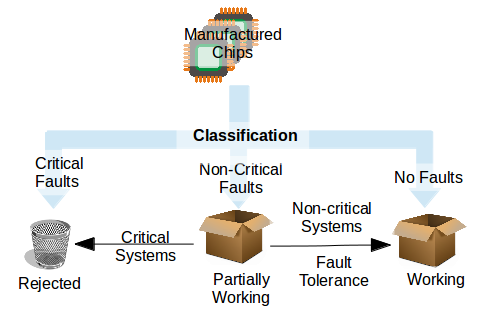
\includegraphics[scale=0.55]{figures/proposedflow.png}
    \caption{Proposed classification flow for VLSI Chips}
    \label{fig:proposedflow}
  \end{center}
\end{figure}

With scaling is expected that, non-critical failures (\emph{i.e.} failures due to transient faults) will constitute majority of failures \cite{Constantinescu2003}. Hence a significant yield loss can be avoided by using the method proposed above. This can be achieved if we are able to classify faults as permanent, transient and intermittent, then reject circuits with permanent and intermittent faults, while retaining chips transient faults. Such classification can also help the designers with statistics about failures, which can be useful to find underlying defect mechanism, resulting in improvement of product quality.

Classification of faults into such categories is difficult as intermittent faults and transient faults manifest similarly. This is even more apparent, as systems move to lower technology nodes. It then becomes difficult to classify faults with traditional approaches, as criteria used for classification are not conclusive. This ambiguity, and the fact that problem at hand is changing as technology continues to evolve, calls for an alternative approach, which is adaptive and where a system can classify faults accurately.

Machine learning techniques are shown to be useful in cases where it is difficult to express knowledge in terms of fixed set of rules. Machine learning approaches have shown that the lack of knowledge can be covered up with data. In our case, the ambiguity of the classification rules can be covered up by storing past classification decisions and \enquote{learn} from those for accurate classification. The primary focus of the thesis is to explore the possibility of fault classification by using machine learning methods.

\section{Thesis Organization}
This thesis report is organized as follows:
\begin{description}
\item[Chapter~\ref{chap:chapter2} -- \nameref{chap:chapter2}:] First part of this chapter defines the fault taxonomy used for classification. It covers the definition, sources and fault models used for each of fault types. It also notes the characteristics for fault types used to derive feature in later chapters. Second part of the chapter covers related work done to classify faults in computing systems and on VLSI chips. Third part presents a brief account of fault diagnosis and diagnostic parameters.

\item[Chapter~\ref{chap:chapter3} -- \nameref{chap:chapter3}:] This chapter covers some basics of machine learning. It explains supervised and unsupervised approaches for machine learning. A brief survey of some of popular machine learning algorithms are covered in this chapter, along with their training procedures and advantages and disadvantages of using each of them.
 
\item[Chapter~\ref{chap:chapter4} -- \nameref{chap:chapter4}:] A detailed account of the problem definition is covered in the first part of this chapter. Second part covers feature selection for classification and their extraction methods. Selection criteria for machine learning algorithm used for classification is explained in later part of the chapter.

\item[Chapter~\ref{chap:chapter5} -- \nameref{chap:chapter5}:] This chapter starts with assumptions and experimental setup to generate sample population and test data for learning is explained in this chapter. Rest of the chapter focuses on procedure to train the classifier and using the same for fault classification.

\item[Chapter~\ref{chap:chapter6} -- \nameref{chap:chapter6}:] Results obtained using the techniques described in chapter~\ref{chap:chapter4} and~\ref{chap:chapter6} are presented in this chapter.

\item[Chapter~\ref{chap:chapter7} -- \nameref{chap:chapter7}:] This chapter concludes the thesis and summarizes possible applications of method suggested in this thesis and future work.
\end{description}

%Die Angabe des schlauen Spruchs auf diesem Wege funtioniert nur,
%wenn keine Änderung des Kapitels mittels den in preambel/chapterheads.tex
%vorgeschlagenen Möglichkeiten durchgeführt wurde.
\chapter{Faults in VLSI Systems}
\label{chap:chapter2}
%\vspace{-3cm}
%\vspace{2cm}

Reliability is always a cause of concern during chip manufacturing. A manufactured chip needs to function correctly not just during post-manufacturing tests but during the complete lifespan of the chip. Typical lifespan for a chip designed for commercial purpose is defined as 11.4 years or 100,000 hours \cite{kishore2009}. Failure rate of ICs with respect to time is shown in figure~\ref{fig:bathtubcurve}, typically known as \emph{bathtub curve}.

\begin{figure}[h]
  \begin{center}
    \captionsetup{justification=centering}
    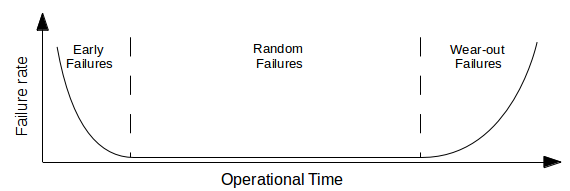
\includegraphics[scale=0.5]{figures/bathtubcurve.png}
    \caption{Bathtub Curve}
    \label{fig:bathtubcurve}
  \end{center}
\end{figure}

The first region of the graph is called early failures or \emph{infant mortality region}. The second region is the lifetime of the device when random failures occur. The error rate in this region is low and constant. Third region of the graph is wear-out and is caused by failures at the end of the useful life \cite{kishore2009}. It can be expected that the ICs will not enter this region due to technology advances and obsolescence. This makes the first region important from the view of product quality and thus it is important to detect faults at manufacturing level. 

Incorrectness of a VLSI system can be described as a fault, defect or an error. A \emph{defect} in an electronic system is an unintended difference between implemented hardware and its design \cite{Agrawal2000}. Defects can occur either during the manufacturing process or lifetime of the device. An \emph{error} is said to have occurred when an unintended output signal is produced by the system. An error is essentially manifestation of a defect. For the purpose of analysis, a defect is modeled as a \emph{fault}, which is simply representation of defect at abstracted function level.

\begin{figure}[h]
  \begin{center}
    \captionsetup{justification=centering}
    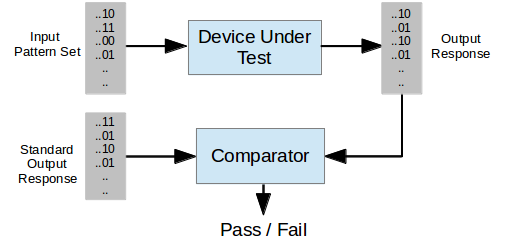
\includegraphics[scale=0.75]{figures/vlsitesting.png}
    \caption{Typical test flow for VLSI Chips}
    \label{fig:vlsitesting}
  \end{center}
\end{figure}

The figure~\ref{fig:vlsitesting} shows how faulty chips are identified. To decide whether the Device under Test (DUT) is working properly, a set of input stimuli called \emph{test pattern set} is applied to the DUT. \emph{output response} is observed and is then compared standard output. If these outputs do not match then the chip is said to be faulty.

The sources of the fault can be internal or external. When healthy chips fail due external mechanisms like $\alpha$-particle strikes, they are thrown away which contributes to yield loss. Thus to maintain product quality and to reduce yield loss, it is important classify the faults. Section 2 of this chapter describes a taxonomy for such classification according to their sources and characteristic. It also focuses on various fault models that can be used to analyze these faults. The existing techniques for such fault classification are explained in section 3. The last section of this chapter explains diagnostic techniques and how they can used to classify faults.

\section{Fault Taxonomy}
\label{sec:secft}
According to the sources of faults, they can be classified into three types: \emph{permanent}, \emph{intermittent}, and \emph{transient}. Permanent faults reflect irreversible physical changes. Intermittent faults occur because of unstable or marginal hardware and can be activated by environmental changes, like higher or lower temperature and voltage. Transients occur because of temporary environmental conditions \cite{Constantinescu2003}. The likelihood of these faults is expected to be higher as increasingly greater amount of transistors are integrated in smaller area \cite{Constantinescu2007}.

\subsection{Permanent Faults}
Permanent faults are those which occur due to permanent physical changes on chip. These faults generally occur due to issues in manufacturing process, however they can also occur during operational lifetime of the circuit, especially when circuit is old and starts to wear-out \cite{Lehtonen2009}.

\subsubsection{Sources of Permanent Faults:}
\paragraph{Manufacturing process:}
So-called \emph{spot defects} can occur during manufacturing of a VLSI chip, and take form of either missing or extra material. Such a defect can cause an unwanted short or open between nodes or make an unintended multi-terminal transistor,leading to changed circuit topology. These defects mainly arise from some contamination, usually in form of dust particles or liquid droplets deposited on the wafer surface during some fabrication step \cite{Khare1996}. Also missing or excess metal may cause unwanted capacitance and resistance respectively resulting in delay lines \cite{Wagner1995}.

\paragraph{Operational failures:}
\emph{Electromigration} (EM) is defined as mass transport of metal atoms created by collision of electrons \cite{Ghate1982}. This movement of material will result in voids or hillock growth as in figure~\ref{fig:mfgdefects} \cite{Lehtonen2009}, which can result in open circuit or short between adjacent tracks \cite{AnalogDevices2000}. With lower technology nodes, the wire widths are also getting smaller making EM a serious problem. 

\begin{figure}[h]
  \begin{center}
    \captionsetup{justification=centering}
    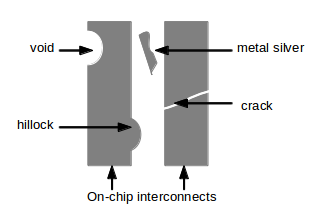
\includegraphics[scale=0.75]{figures/mfgdefects.png}
    \caption{Manufacturing defects as sources for intermittent and permanent faults }
    \label{fig:mfgdefects}
  \end{center}
\end{figure}

\subsubsection{Characteristics of permanent faults:}
\begin{itemize}
	\item Once permanent fault appears in the system, it does not go away.
	\item The faults are localized on the chip. They will affect the same set of primary outputs (POs).
	\item Permanent faults are reproducible and provide a predictable output response.
 	\item Permanent faults only go away once the offending component is replaced \cite{Constantinescu2007}.
\end{itemize}

\subsubsection{Fault models for permanent faults:}
\paragraph{Stuck-at fault model:}
Stuck-at fault models are the most simplest fault models. Due to its simplicity and ability to explain many defects accurately, they are widely used \cite{Larsson2006}. It assumes that the fault location has a fixed logical value, either stuck-at 0 or stuck-at 1. These can be seen as short to ground or short to power supply respectively. When it is assumed that there is only one fault in the circuit at a time then \emph{single stuck-at} (SSA) model is used, otherwise in case of multiple defects \emph{multiple stuck-at} model is used. In this thesis we have assumed that there is only one fault active in the circuit at a given time; hence we have used SSA model for our analysis.

\paragraph{Wired AND/OR fault model:}
Unlike stuck-at, \emph{bridge fault} models a short between signal lines. \emph{Wired AND/OR} fault model is type of bridging fault model. These models are used to describe logic behavior of two nodes that are shorted in the circuit. Wired AND model assumes that the faulty node of the bridge always has value 0, whereas wired OR model assumes faulty node has value 1. 

\paragraph{Delay fault model:}
\emph{Delay fault} model is used to model timing related faults. Delay testing is required for modern VLSI systems running at high frequencies, as even minor timing violations can lead to system performing out of specifications \cite{Larsson2006}. There are two was to realize delay viz. \emph{Gate delay} and \emph{Path delay} models. Gate delay model assumes that the delay is only between input and output of individual logical gates on chip. In contrast, path delay models assume that the delay is spread over complete path from input to output. 

\subsection{Intermittent faults}
\label{sec:secif}
Intermittent faults are those caused by marginal or unstable hardware and are activated when certain conditions like voltage, temperature or frequency are met \cite{Constantinescu2003, Lehtonen2009}. Intermittent faults often precede occurrence of permanent failures \cite{Lehtonen2009}.

\subsubsection{Sources of intermittent faults:}
\paragraph{Manufacturing defects:}As illustrated in figure~\ref{fig:mfgdefects} \emph{metal silvers} are stray pieces of metal on die due to some process imperfections. In certain conditions like increase in temperature, the metal may expand and touch the interconnects creating a short. In some cases the short might cause a current surge, damaging the circuit and can manifest into a permanent fault \cite{Hawkins2003}. Similarly cracks, as shown in same figure can continue to work normally at design temperature but at low temperatures can cause open circuits.

\paragraph{Technology scaling:} With technology scaling, the supply voltages are also lowered down, which results in degraded noise tolerance \cite{Lehtonen2009}. Also the reduced thickness of oxide layers may result in current leakage, with a mechanism known as soft breakdown (SBD) \cite{Stathis2001}. In such a breakdown, current fluctuates creating intermittent fault, without causing thermal damage \cite{Stathis2001, Constantinescu2007a, Constantinescu2007}.

\subsubsection{Characteristics of intermittent faults:}
\begin{itemize}
	\item Once intermittent fault appears in the system, its probability of recurrence increases \cite{Bondavalli2000}.
	\item The faults are localized on the chip. They will affect the same set of primary outputs (POs).
	\item Intermittent faults not reproducible every time however they provide a predictable output response.
 	\item Intermittent faults only go away once the offending component is replaced \cite{Constantinescu2007}.
	\item Intermittent faults have tendency to occur in bursts \cite{Constantinescu2007, Constantinescu2003}.
\end{itemize}

\subsubsection{Fault models for intermittent faults}
Intermittent faults can be modeled as conditional stuck-at faults, which are traditional stuck-at faults activated by trigger condition. The activation condition can be expressed as boolean function and may depend on timing or environmental conditions \cite{Holst2009}.

\paragraph{High frequency power droop:}A high frequency power droop occurs when multiple cells on a chip connected to same power grid segment switch in same direction, increasing their current demand cause power starvation in some other part of chip. This fault is modeled as a set of aggressor lines $a_1,a_2,...$ and a victim line $v$ \cite{Polian2007}. The fault occurs on victim line, due to presence of aggressor lines.

\subsection{Transient faults}
\label{sec:sectf}
Transient faults are temporary deviations of normal circuit function caused by some temporary environmental factors or some external phenomenon. They are called soft errors as they do not do any permanent damage to the chip. A \emph{single-event upset} (SEU), which is change in value of single bit, is the most common manifestation of transient faults.

\subsubsection{Sources of transient faults}
\paragraph{Particle strikes:}When an $\alpha$-particle, proton or a neutron passes through a semiconductor material and starts to loose energy, it frees electron-hole pairs along its path \cite{Dodd2003}. If this material happens to be a reversed biased p-n junction, it can result in significant transient currents to bring about an SEU. Hence with scaling to lower technology nodes, it is very likely that probability of such SEUs will increase.

\paragraph{Other sources:} \emph{Electromagnetic interference} caused by sources emitting high energy signal may interfere with working chip to bring about SEUs. \emph{Electrostatic discharge} due to users releasing static charge can also affect chips to cause transient faults.

\subsubsection{Characteristics}
\begin{itemize}
	\item Transient faults are non-deterministic faults.
	\item These faults are not localized hence can affect any of the POs.
	\item Transient faults are not reproducible.
 	\item Replacing offending component may not make transient faults to go away \cite{Constantinescu2007}.
	\item Transient faults are isolated incidences of error occurrence, they usually do not occur in bursts like intermittent faults \cite{Constantinescu2007, Constantinescu2003}.
\end{itemize}

\subsubsection{Fault models for transient faults}
One of the ways  to model transient fault is to implement a conditional stuck-at fault, at multiple fault location and to use a deterministic function to trigger the fault \cite{Holst2009}


\section{Fault Classification}
\label{sec:secfc}
Test flows like one shown in figure~\ref{fig:vlsitesting} are able to distinguish between faulty and healthy chips. A better approach in \cite{DeKleer2009} is able to distinguish permanent faults from faults with non-deterministic behavior. However the traditional post-manufacturing tests still work same way as shown in figure~\ref{fig:traditionaltestflow} \cite{Weste1985}. 

\begin{figure}[h]
  \begin{center}
    \captionsetup{justification=centering}
    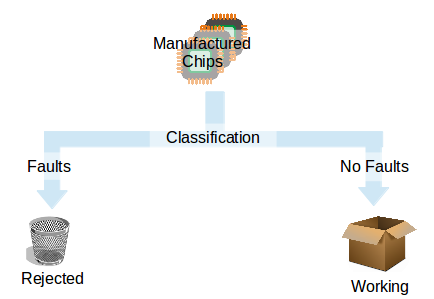
\includegraphics[scale=0.75]{figures/traditionaltestflow.png}
    \caption{Traditional flow for fault classification}
    \label{fig:traditionaltestflow}
  \end{center}
\end{figure}

With advances in manufacturing processes number of permanent faults are reducing \cite{kishore2009}, while on the other hand the impact of soft-errors and other non critical failures is increasing \cite{Constantinescu2003}. Some studies have indicated that up to 80\% failures can be attributed to SEUs \cite{Iyer1986, Dharchoudhury1994, kishore2009}, which suggest that these cases will result in unnecessary yield loss. This section describes a few techniques to discriminate between different error categories described earlier in the chapter. As the error categories are similar in characteristics to those observed on PCs or workstations, the approaches used for their classification also provide a few pointers towards fault classification in VLSI systems. 

In \cite{Lin1990} a mechanism to classify between transient and intermittent faults is explained for error log analysis. In a technique called \emph{Dispersion Frame Technique} (DFT), inter-arrival time in between successive error events of same error types is used to determine type of fault in the system. Heuristics are applied to determine closeness in time and affected area which are then considered as parameters to decide whether the error is of the same type.

Authors in \cite{Iyer1990} use a similar technique to identify persistent failures in the system. Here they have used error rates to build up correlation using simple probabilistic techniques between error records, leading to a set of symptoms which may suggest a common cause (permanent errors).

A probabilistic approach is considered in \cite{Pizza1998}, which updates probability of module being affected by permanent fault. It then weighs the consequences of actions performed by a faulty module vs. fault-free module uses Bayesian inference to discriminate between permanent and transient errors

\subsection{Fault Classification Techniques for VLSI Systems}
Historically a lot of work has been done to analyze impact of different types of faults on VLSI systems \cite{Constantinescu2003,Constantinescu2007,Dodd2003} and to classify them \cite{Savir1980, Espinosa2013, Bondavalli2000, DeKleer2009}. The most popular techniques to classify transients from other types of faults are grouped under a family called $\alpha$-count techniques \cite{Bondavalli2000}. In a scheme called\emph{single threshold $\alpha$-count techniques}, a single threshold is established and if error count exceeds this threshold then fault is classified as permanent or intermittent, whereas a smaller non-zero value indicates presence of transient faults. In an other variant of the same called \emph{dual threshold $\alpha$-count techniques}, two thresholds are established. If error count exceeds first threshold then component is assigned a restricted functionality and when it exceeds the second threshold it is taken out of service, like single threshold. However a component in between thresholds can be taken in full service once its error count is lowered than first threshold.

\section{Fault Diagnosis}
\label{sec:secfd}
\emph{Diagnosis} is the process of locating faults in a physical chip at the various levels down to real defects. In traditional fault-dictionary based diagnosis, we are given two sets of data, a \emph{predicted output} $P$ which is set of outputs when fault a particular fault is active in the system, a \emph{measured set} $M$, which is observed fault behavior and corresponding fault $ f_i \in \{f_1,f_2,...,f_n\} $. When the two sets match i.e. $P = M$ the corresponding fault is diagnosed to be active . When $P \neq M$ then logic diagnosis tries to find best fitting explanation. However it is practically infeasible to construct such fault dictionaries for modern circuits, as the fault dictionary should consist of all possible faults and their combinations \cite{Wang2010}. 

An adaptive approach which does not use fault dictionaries called \emph{Partially Overlapping Impact couNTER} (POINTER) for diagnosis is described in \cite{Holst2009}. This approach uses test pattern sets with \emph{Single Location At a Time} (SLAT) property \cite{Bartenstein2001} to diagnose faults present in the circuit. The author in \cite{Holst2009} defines a \emph(Fault Machine) (FM),i.e. a circuit with stuck-at fault injected. As shown in figure~\ref{fig:evidance} a set of tuple parameters called
\emph{evidance} is defined as,

$e(f,T) = (\sigma_T, \iota_T, \tau_T, \gamma_T)$, where for all patterns $t \in T$

\begin{itemize}
	\item $\sigma_T$ is sum of number of failing outputs where Device Under Diagnosis (DUD) and FM match
	\item $\iota_T$ is sum of number of outputs which fail in FM but are correct in DUD.
	\item $\tau_T$ is sum of number of outputs which fail in DUD but are correct in FM.
 	\item $\gamma_T$ is the sum of maximum of $\iota_t $ and $\tau_t$ for every pattern $t \in T$.
\end{itemize}

\begin{figure}[h]
  \begin{center}
    \captionsetup{justification=centering}
    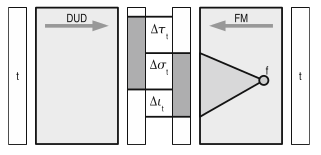
\includegraphics[scale=0.75]{figures/evidance.png}
    \caption{Definition of evidance}
    \label{fig:evidance}
  \end{center}
\end{figure}

These parameters vary depending on the type of fault present in the circuit. The use of these parameters to classify faults is explained in section <section reference: feature selection> of this report.  



%Die Angabe des schlauen Spruchs auf diesem Wege funtioniert nur,
%wenn keine Änderung des Kapitels mittels den in preambel/chapterheads.tex
%vorgeschlagenen Möglichkeiten durchgeführt wurde.
\chapter{Machine Learning For Classification}
\label{chap:chapter3}
%\vspace{-3cm}
%\vspace{2cm}
An \emph{algorithm} is a set of instructions used to convert input values to an output, based on certain rules. Consider an example where we need to find all even numbers from a dataset. Here, we can set up a \emph{rule} that if a number is completely divisible by two then it should be included in the output dataset, otherwise not. Naturally, as there can be more than one way to solve a problem, there can be more than one algorithm to solve it. However, there are certain examples where formation of set of rule is practically infeasible. For an example, consider a handwriting recognition software used to scan handwritten forms. Figure~\ref{fig:charrec} illustrates the problem at hand, where a simple character can be written in a number of ways. It is interesting to note that humans are able to read this data without a trouble, but it is really difficult to infer a set of rules which would result in an accurate recognition with help of an algorithm. Machine learning is employed in such cases. Specifically \emph{Machine Learning} (ML) is programming computers to optimize a performance criterion (e.g. character recognition) using example data or a past experience \cite{Alpaydin2004}. 

\begin{figure}[h]
  \begin{center}
    \captionsetup{justification=centering}
    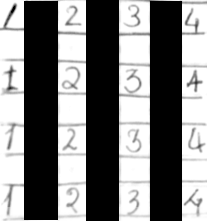
\includegraphics[scale=0.5]{figures/charrec.png}
    \caption{Example of Machine Learning: Character recognition}
    \label{fig:charrec}
  \end{center}
\end{figure}

In case of a handwriting recognition system, an \enquote{example data}, in the form of images of handwritten characters with their \emph{labels}, \emph{i.e.} a number or an alphabet, which each image represents, is collectively referred to as a \emph{training set}, and is used to teach machine learning how a character with the given label would look like, so that ML can recognize when it encounters similar data in the future. Machine learning can be applied in a wide range of applications, where it is not possible to the express human expertise, but a large amount of sample data is available. Typical applications of machine learning include computer vision, pattern recognition, spam filtering, search result optimization etc. 

\section{Types of learning algorithms}
\label{sec:secmltypes}
Based on whether we know labels for the data, ML algorithms can be can be classified in two major categories - supervised learning and unsupervised learning. 

\emph{Supervised learning} algorithms are used when labels of the data to be are known. A spam filter is a good example where supervised learning can be used for \emph{classification}. Here we know an email received is either "spam" or "not-spam", these categories can be used as labels for the sample population and learning algorithm can classify within these two type.  One more application of supervised learning is to predict a numerical value in \emph{regression}. Consider a problem to predict value of a used property, the input parameters in this case are the initial value, year of the construction, size of the property, the locality and so on, whereas the output is the current resale value. one can construct a training set of known resale values and receptive values of input parameters and train the leaning algorithm to predict other inputs. To generalize, aim in supervised learning is to learn mapping from input to output whose correct vales are provided by supervisor \cite{Greene2008}.

\emph{Unsupervised learning} is used in classification problems where the labels for the data are not known. An example of such problem is data clustering \cite{Jain1988}. One of applications of this is to cluster news reports which belong to the same category like sport, science, art and so on. The number and the labels of categories in this case are not defined, and the machine learning application needs to cluster articles based on some common words, and provide the supervisor data, which he may use to label the clustered groups. The aim in supervised learning it to find out regularities or correlation the  input data, without explicit need of a supervisor \cite{Marinai2008}

In case of fault classification, a classification taxonomy has been discussed in earlier chapter. The sample population, which we would generate in our case will contain labels. This makes our case as supervised classification problem. In following subsection, we define the basic terms as applied to case of supervised learning.

\section{Basic terms in supervised machine learning}

A \emph{feature} $(x_i)$ is a result of measurement made on a unit input data. Generally, a set of features $(\boldsymbol{x})$ is needed to characterize a unit of input data and is expressed as,
\[ \boldsymbol{x} = \left[ x_1, x_2, \ldots x_m \right]^T \]  
Its label $l$ denotes the class $C_i \in \{C_1, C_2 \ldots C_k\}$ it belongs to and it is denoted as,
\[ l_i = \left\{ \begin{array}{ll}
         1 & \mbox{if $\boldsymbol{x} \in C_i$};\\
         0 & \mbox{if $\boldsymbol{x} \in C_j, j \neq i$}\end{array} \right. \] 
The \emph{training set} $X$ is then defined as a set containing $N$ values of such examples,
\[ X = \{\boldsymbol{x}^t , \boldsymbol{l}^t \}_{t=1}^N  \]
The aim for machine learning algorithm is to learn data and their labels in the training set and then classify the new examples $\boldsymbol{x}$ by estimating the value of $C(\boldsymbol{x})$. To achieve this, the algorithm tries to find out a hypotheses for every class, $h_i, i \in\{1,2, \ldots k\}$ from a set of all possible hypotheses such that,
\[ h_i(\boldsymbol{x}) = \left\{ \begin{array}{ll}
         1 & \mbox{if $\boldsymbol{x} \in C_i$};\\
         0 & \mbox{$\boldsymbol{x} \in C_j, j \neq i$}\end{array} \right. \] 
The \emph{empirical error} after training is calculated as,
\[ E(\{h\}_{i=1}^k|X) = \sum\limits_{t=1}^N \sum\limits_{i=1}^k | h_i(\boldsymbol{x}) \neq l_i^t ) | \]

Figure~\ref{fig:mlfitting} shows two possible hypotheses $h_1$ , $h_2$ and the actual boundary of classification $C$. For a simple 2-class classification problem, both the hypotheses have the same value of empirical error. If we choose hypothesis $h_1$ then the examples which lie in region between $h_1$ and $C$ will get incorrectly classified and this is called as \emph{overfitting}. On the other hand, if we choose $h_2$ then same will happen for examples in the region between $C$ and $h_2$, called \emph{underfitting}. To check if overfitting or underfitting is has occurred, typically one more labeled dataset called as \emph{cross-validation set} is picked. The empirical error is then calculated over this set and hypotheses obtained during training and the hypothesis with least value of error is then selected. 

\begin{figure}[h]
  \begin{center}
    \captionsetup{justification=centering}
    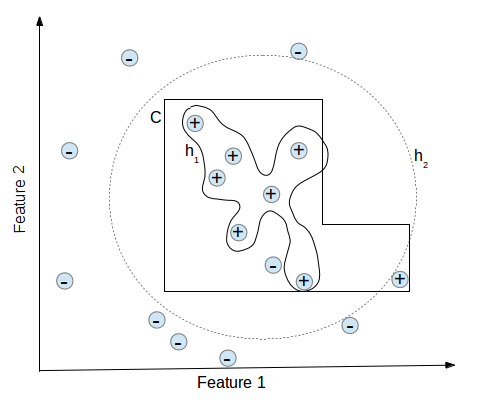
\includegraphics[scale=0.45]{figures/mlfitting.png}
    \caption{Example of overfitting and underfitting}
    \label{fig:mlfitting}
  \end{center}
\end{figure}
In this report, the term \emph{sample population} collectively for the training set and the cross-validation set.

\section{Machine Learning Algorithms for Classification}
\label{sec:c3mlclassification}
This section provides a brief overview of some of the most frequently used machine learning algorithms for the classification problem. It includes advantages and disadvantages for individual algorithms.

\subsection{Naive Bayes}
Naive Bayes is one of the simplest algorithms for learning, more interestingly in some cases it may outperform most of the sophisticated learning algorithms \cite{John1995}. The naive Bayes uses maximum-likelihood estimation to classify new examples. It is based on the Bayes' theorem which states,
\[ P(A|B) = \frac{P(B|A) \times P(A)}{P(B)} \]
Where $P(A)$, $P(B)$ being the probabilities of A and B, and $P(A|B)$ and $P(B|A)$ are conditional probabilities of A, given B and B, given A respectively.
 
During the training of the naive Bayes, the probability of finding an example of each class in the sample population is calculated and stored as the \emph{prior} probability for that class. It also calculates probability for instances $\boldsymbol{x}$ given its class $c$. Under the assumption that attributes in $\boldsymbol{x}$ are independent, it simply becomes a product of probabilities of each single attribute \cite{Williams2006}.
Hence Bayesian theorem, when applied to classification problem using Naive Bayes, becomes
\[ P(C_i|\boldsymbol{x}) = \frac{P(\boldsymbol{x}|C_i) \times P(C)}{P(\boldsymbol{x})}\]
The probability $P(C_i|\boldsymbol{x})$ is referred to as \emph{posterior} probability. A class $C_i$ is chosen if $P(C_i|x) = \max\limits_{k} \{ P(C_k|x)\}$, \emph{i.e.} the class with highest posterior probability.

A clear advantage of using the naive Bayes is that, it is fast to train and fast to classify the data. This is because it needs to scan the database to compute probabilities and store it in a table during training and use this table to classify future examples. Also the naive Bayes is inherently more robust against irrelevant features \cite{Kim2008}, as the likelihood of a class is product of probabilities of each single attribute. On the other hand for prior probabilities to be realistic, the sample population needs to be truly representative of the actual data. Another major disadvantage is that the classifier assumes features to be independent of each other. However in many cases Naive Bayes classifier performs reasonably well even in cases where features are dependent on each other \cite{John1995, Williams2006}.

\subsection{Decision Trees}
\emph{Decision trees} are hierarchical models, wherein each step is a simple threshold-test function of nominal value of a feature against a fixed threshold value \cite{Kotsiantis2013}. The steps in the hierarchy are called as \emph{decision nodes} and a \emph{test} is implemented in the form of a function on features $\boldsymbol{x}$ of an example, with discrete outcomes represented as branches. These nodes apply tests recursively on a feature or a set of features of the  example data, until it flows down the tree and hits a \emph{leaf node}, which represents the output (class in case of classification) \cite{Alpaydin2004}. A simple decision tree is illustrated in figure~\ref{fig:desctree}.

\begin{figure}[h]
  \begin{center}
    \captionsetup{justification=centering}
    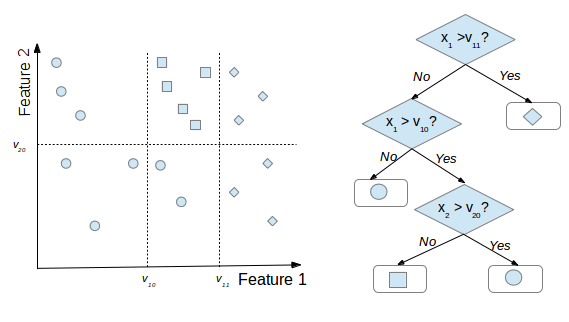
\includegraphics[scale=0.65]{figures/desctree.png}
    \caption{Example of decision tree}
    \label{fig:desctree}
  \end{center}
\end{figure}

In terms of a computer program, this algorithm devices a set of rules which can be interpreted as nested \texttt{IF-ELSE} structure. The \emph{decision tree learning} algorithms are used to derive decision trees. ID3, C4.5 are some examples of these algorithms \cite{Mitchell1997}. ID3 \cite{Quinlan1986} is the simplest of these algorithms. In the case of decision trees, training is to choose features which provides the most information about training set. It then constructs tree using top-down approach. Other advanced algorithms like RIPPER \cite{Cohen1995} build upon the same approach and then employ \emph{pruning} to reduce the training error.

Decision trees use a \enquote{white-box} approach, wherein the internal decision making and structure of tree is visible to user. This also makes decision trees easy to visualize and interpret \cite{Kotsiantis2013}. Decision trees also perform a feature screening to put less informative features near leaf nodes, by its construction.A disadvantage of decision trees is that they can create over-complex trees that do not generalize the data well, \emph{i.e.} the overfitting of data. The problem of learning decision trees is known to be NP-complete hence its worst-case training speed can be slow \cite{Hyafil1976}.

\subsection{Multi-Layer Perceptrons}
\emph{Multi-Layer Perceptrons} (MLP) is a type of artificial neural network models and has been in use since the early 80's. In this model, each feature and output are represented as nodes, and feature nodes in each layer are connected to the upper layer using weights or \emph{synapses}. Figure~\ref{fig:perceptron} is an example of a simple, two layered perceptron. Inputs $x_1, x_2 \ldots x_k$ are features and $x_0 = +1$ is a \emph{bias element}, used to make model more general by allowing user to fine-tune the the output by shifting the output function. $\boldsymbol{a,b}$ are matrices of weights on the synapses in the first to the hidden layer and the hidden layer to the output, respectively.

\begin{figure}[h]
  \begin{center}
    \captionsetup{justification=centering}
    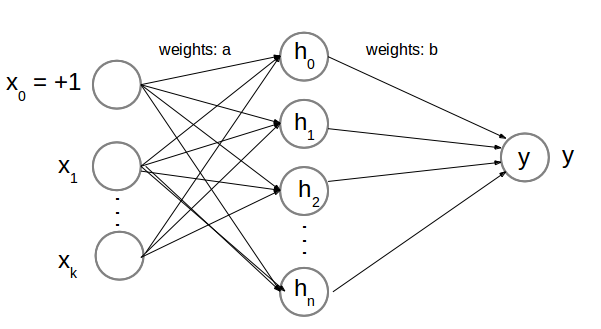
\includegraphics[scale=0.45]{figures/perceptron.png}
    \caption{Two layered perceptron}
    \label{fig:perceptron}
  \end{center}
\end{figure}

The output of perceptron in figure~\ref{fig:perceptron} can be represented mathematically as
\[ y = \sum\limits_{j=0}^n b_j (\sum\limits_{i=1}^k (a_{ij}x_i + a_0))\]
During the training of a perceptron, the training algorithm will try to find the appropriate connecting weights. Multiple layers of perceptrons can be constructed by implementing a hidden layer of nodes between features and output, by doing so one can implement non-linear output functions. The degree of non-linearity depends on the number of hidden layers. Back-propagation algorithm \cite{Rumelhart1985} is one of commonly used algorithm for training MLPs. It works by calculating error correlations at each output and use these to calculate the error terms in previous layers and so on. The error terms are then used to adjust weights of the individual synapses. 

The error function in this case is defined as,

\[ E(\boldsymbol{a},\boldsymbol{b}|X) = \frac{1}{2} \sum\limits_{t} (l^t - y^t)^2\]

The gradient of this error function is calculated during back-propagation, and weights are updated once the gradient function reaches a local minimum.

Once trained, MLPs are able to classify data fast. They can implement higher order polynomial functions and are flexible and powerful due to well researched mathematical background and variety of training algorithms available, which can be selected according to the application and the amount of data available. A disadvantage is that the network needs to be completely re-trained when new training data is to be added. Selection of features also has a profound impact on the performance of MLPs \cite{Kavzoglu2002, El-Khatib2010}.

\subsection{Support Vector Machines}
\label{mltypes:svm}
\emph{Support Vector Machines} (SVMs) have existed for a long time, but the research on these gained particular momentum since Vapnik \cite{Vapnik1995} evaluated these methods in his book on statistical learning theory. SVM belongs to the class of linear classifiers. In higher dimensions, SVM tries to divide the feature space using decision hyperplanes. However, as there can be several planes that divide feature space, SVM selects the plane with maximum distance from support vectors. Figure~\ref{fig:svm1} shows a case where two possible lines divide feature space, $h_1$ and $h_2$. SVM will choose $h_2$ as the \emph{decision boundary} or the \emph{discriminant function} as it provides maximum margin for the classification. The examples with least distance from the decision hyperplane are called \emph{support vectors}.

\begin{figure}[h]
  \begin{center}
    \captionsetup{justification=centering}
    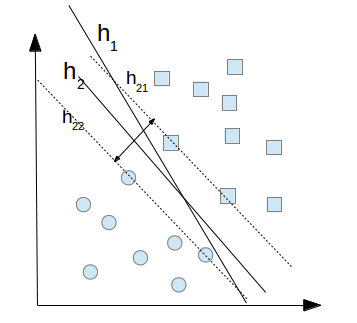
\includegraphics[scale=0.45]{figures/svm1.png}
    \caption{SVM with linear decision boundary}
    \label{fig:svm1}
  \end{center}
\end{figure}
The linear discriminant function used in this case can be expressed as,
\[g(x) = \boldsymbol{w^T}\boldsymbol{x} + w_0 \]
Where $w_0$ denotes a bias, and the vector $\boldsymbol{w}$, called weight vector, is the distance of respective hyperplanes passing through support vectors from the origin.

Referring to figure~\ref{fig:svm1}, hyperplane $h_2$ is actually a result of two hyperplanes, defined by the respective support vectors of two classes. Let $h_{21}$ and $h_{22}$ represent these hyperplanes	such that:
\[\begin{array}{ll} 
h_{21}: \boldsymbol{w^T}\boldsymbol{x} + b = 1 & \mbox{when label is +1};\\
h_{22}: \boldsymbol{w^T}\boldsymbol{x} + b = -1 & \mbox{when label is -1}
\end{array} \]

However as illustrated in the figure~\ref{fig:svm2} the feature space may not be linearly separable at all. In these cases SVM uses \emph{kernel trick} to achieve linearly separable kernel space. The idea behind kernel trick is to apply a function $\phi$ to transform all points in the feature space to a higher dimension, so that resulting feature space is linearly separable. After transformation, the regular SVM algorithm is used for classification.

\begin{figure}[h]
  \begin{center}
    \captionsetup{justification=centering}
    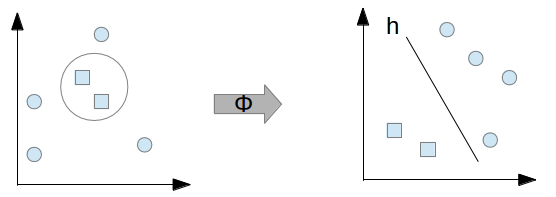
\includegraphics[scale=0.50]{figures/svm2.png}
    \caption{Kernel trick for SVM}
    \label{fig:svm2}
  \end{center}
\end{figure}

This makes the linear discriminant used of the form,
\[\boldsymbol{y} = \boldsymbol{w^T}\phi(\boldsymbol{x}) + w_0 \]

where $\phi$ denotes the function used to convert the non-linear feature space to linear one.

Let $||\boldsymbol{w}||$ denote the distance between these hyperplanes, C a constant to adjust variance and to minimize the training error $\xi$ . Then the training of SVM is to find a maximum margin hyperplane, which can be viewed as an optimization problem \cite{Vapnik1995, Chang2011},
\[\begin{array}{ll} 
 \min\limits_{\boldsymbol{w},\xi,w_0} &\frac{1}{2} ||\boldsymbol{w}||^2 + C \sum\limits_{i=1}^n \xi_i \\
 \mbox{subject to} & l^t(\boldsymbol{w^T}\phi(\boldsymbol{x}) + w_0) 
\end{array}\]

This QP may be difficult to solve as function $\phi(\boldsymbol{x})$ can be high in dimensions. Making the mapping used computationally expensive \cite{Ben-Hur2010}.

To solve this, suppose $\boldsymbol{w}$ can be expressed as $\boldsymbol{w} = \sum\limits_{i=1}^n \alpha_i\boldsymbol{x_i}$ (dual of this problem), and also define a \emph{kernel function},
\[K(\boldsymbol{x},\boldsymbol{x_i}) = \phi(\boldsymbol{x})\phi^T(\boldsymbol{x_i})\]
 Substituting this in minimization problem reduces the dimensionality back to the original.

Most commonly used kernels are:
\begin{description}
  \item[Linear] $K(\boldsymbol{x},\boldsymbol{x_i}) = \boldsymbol{x}^T\boldsymbol{x_i}$
  \item[Polynomial] $K(\boldsymbol{x},\boldsymbol{x_i}) = \gamma(\boldsymbol{x}^T\boldsymbol{x_i}+r)^d, \gamma > 0$
  \item[Radial Basis Function (RBF)] $K(\boldsymbol{x},\boldsymbol{x_i}) = \mathrm{e}^{-\gamma||\boldsymbol{x}-\boldsymbol{x_i}+r)||^2}, \gamma > 0$
  \item[Sigmoid] $K(\boldsymbol{x},\boldsymbol{x_i}) = \tanh(\gamma\boldsymbol{x}^T\boldsymbol{x_i}+r)$
\end{description}

$\gamma$, $r$ and $d$ are the kernel parameters.

The advantage of using SVM is its ability to tackle non-linear data. By using a variety of kernels like linear, polynomial, RBF and so on, the user has flexibility to classify the data with non-linear feature spaces \cite {Chang2011}. Handling higher dimensional features spaces is also not an issue, because of the theoretical framework \cite{Vapnik1995} supports an $n$-dimensional space. SVMs also provide a unique solution as the optimality problem is convex, which is an advantage as compared to neural networks, which can provide solutions at a local minimum \cite{Auria2008}. SVM, being a maximum margin classifier, avoids underfitting of data. One the other hand, training an SVM is solving an quadratic optimality problem (known to be NP hard), hence it can take a long time to train when datasets are large. Also, a common disadvantage of SVM is that the model it constructs is a \enquote{black-box} approach to classify the data, specially when the feature set is large \cite{Auria2008}.


%Die Angabe des schlauen Spruchs auf diesem Wege funtioniert nur,
%wenn keine Änderung des Kapitels mittels den in preambel/chapterheads.tex
%vorgeschlagenen Möglichkeiten durchgeführt wurde.
\chapter{Problem Definition and Feature Selection}
\label{chap:chapter4}
%\vspace{-3cm}
%\vspace{2cm}
There are number of methods to separate permanent faults from non-recurring faults as explained in section~\ref{sec:secfc}. However available techniques do not separate faults as permanent, transient and intermittent. This is of particular importance from point of view of reducing yield loss, by including chips which showed only transient faults. Also, if faults can be categorized into these categories, then it gives an additional information to designer about the underlying fault mechanism, so that additional optimization of yield can be achieved. 

The classification approaches explained in section~\ref{sec:secfc} are mostly rule or heuristic based (e.g. threshold value in $\alpha$-counting techniques) and these heuristics or rules will change every time technology is node to lower nodes, hence these rules become obsolete over time. An elaborate analysis is required to update these rules for every product and technology.

Generally speaking, when an intermittent fault occurs in a system, its activation rate is higher than the transient fault rate \cite{Bondavalli2000}. However, as systems are moving to lower technology nodes, transient faults are also on the rise, as explained in section~\ref{sec:secft}. Hence with traditional techniques, it becomes difficult to separate transients from intermittents using $\alpha$-count, as the fault rates for these two types of faults become close to each other.

This calls for an automated and adaptive approach which is independent on product and technology and that can classify faults as intermittent, transient and permanent. 

\section{Machine learning approach for fault classification}

Machine learning has been used in wide variety of classification applications with reasonable accuracy \cite{Pang2002,Nguyen2008,Sebastiani2002, Kotsiantis2007}. As explained in chapter~\ref{chap:chapter3}, machine learning is used when it is not practical to arrive at rules by looking at the data. Machine learning algorithms can be implemented as \enquote{black-box} approach for classification and all user needs to do is adjust a few parameters, depending on machine learning algorithm used. Even parameter searching can be automated and user can fine-tune them for further improvement in accuracy \cite{Hsu2003, Castillo2000}. This makes machine learning a practical and automated approach when large amount of data is available.

Once a feature set is fixed and the required parameters are decided, machine learning algorithms analyze the data to set up a classification model. When a technology node is updated one might have to change the database and train the algorithm again, but the training algorithm takes care of feature space and classification rules, making machine learning approaches adaptive.

Figure~\ref{fig:mlsteps} explains basic steps for classification using machine learning methods.

\begin{figure}[h]
  \begin{center}
    \captionsetup{justification=centering}
    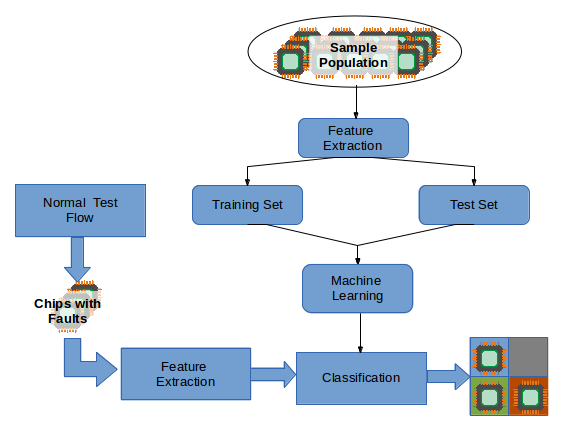
\includegraphics[scale=0.75]{figures/mlsteps.png}
    \caption{Classification of VLSI chips uning machine learning}
    \label{fig:mlsteps}
  \end{center}
\end{figure}

First step in designing a machine learning system for classification is to decide on features, which can be efficiently classify the data. Selection of proper features has the most impact in accuracy of any classifier \cite{Michie1994}. This, along with design of algorithms to extract features from input data is explained in section~\ref{sec:secfs} of this chapter. Next step is to generate sample population and decide on which machine learning algorithm is to be used, covered in next chapter.

\section{Feature Selection}
\label{sec:secfs}
To begin with feature selection, it is important to take a look at all the behavioral characteristics of different types of faults, as covered in chapter~\ref{chap:chapter2}. Table~\ref{tab:charfaults} summarizes all important characteristics to be considered for selection of features. Rest of the section describes features that were selected and algorithms for extraction of those features.

{%
\newcommand{\mc}[3]{\multicolumn{#1}{#2}{#3}}
\begin{table}[H]
 \begin{center}
  \captionsetup{justification=centering}
  \begin{tabular}{lp{4cm}p{4cm}p{4cm}}
    \mc{1}{c}{\textbf{Characteristic}} & \mc{1}{c}{\textbf{Permanent faults}} & \mc{1}{c}{\textbf{Intermittent faults}} & \mc{1}{c}{\textbf{Transient faults}}\\ \hline
    Affected outputs & Affects same set of output pins & Affects same set of output pins & Affects any of primary outputs\\
    Reproducibilty & Reproducible for same test vector & Sometimes reproducible for same test vector depending upon the error activation rate & Not preproducible\\
    Location on chip & Localized to a fault location & Localized to a fault location & Can affect any location on chip\\
    Fault behaviour & Deterministic & Deterministic & Non-deterministic \\ \hline
  \end{tabular}
  \caption{Characteristics of faults in VLSI systems}
  \label{tab:charfaults}
 \end{center}
\end{table}
}%

\subsection{Reproducibility of fault}
Reproducibility of a fault pattern during multiple test runs is defined as maximum number as maximum number of occurrence of same faulty output pattern for a fixed input pattern, and it is denoted by $\epsilon$. 

\begin{figure}[h]
  \begin{center}
    \captionsetup{justification=centering}
    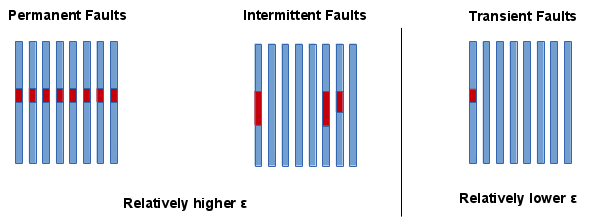
\includegraphics[scale=1.00]{figures/epsilon.png}
    \caption{Expected behavior of $\epsilon$ for different faults}
    \label{fig:epsilon}
  \end{center}
\end{figure}

Algorithm~\ref{alg:epsilon} explains extraction of $\epsilon$. It takes the expected and actual output patterns as inputs. It then checks if any of output patterns was faulty and it calculates maximum occurrences of every faulty pattern for given input pattern and stores in into array. Final value of $\epsilon$ is maximum value of in this array.

\begin{algorithm}[H]
  \caption{Algorithm to evaluate $\epsilon$}
  \label{alg:epsilon}
  \begin{algorithmic}
 \Procedure{ComputeEpsilon}{Expected output pattern array (EX), Observed output pattern array for all test runs (OP)}
 \State $\epsilon$[size(EX)] $\leftarrow$ 0\;
 \State Index $\leftarrow$ 0\;
 \While{Index $<$ size(EX)}
  \If{EX[Index] $\neq$ any pattern of OP[Index][]}
   \State $\epsilon$[Index] $\leftarrow$ max(\Call{SimilarFaultyPatterns}{OP[Index][]})\;
  \Else
   \State $\epsilon$[Index] $\leftarrow$ 0\;
  \EndIf
  \State Index++\;
 \EndWhile
 \State$\epsilon$ $\leftarrow$ max($\epsilon$[])\;
 \State \Return $\epsilon$\;
 \EndProcedure
 \end{algorithmic}
\end{algorithm}

Figure~\ref{fig:epsilon} shows expected behavior of $\epsilon$ for different fault types. Permanent faults are repeatable and value of $\epsilon$ is expected to be equal to the number of test runs for these type of faults. Intermittent faults occur at higher rate than that of transients for a fixed input pattern, hence they are also expected to have somewhat higher value than transient faults. Figure~\ref{fig:epsilonp45k} shows actual values of $\epsilon$ for a simple circuit (p45k).

\begin{figure}[h]
  \begin{center}
    \captionsetup{justification=centering}
    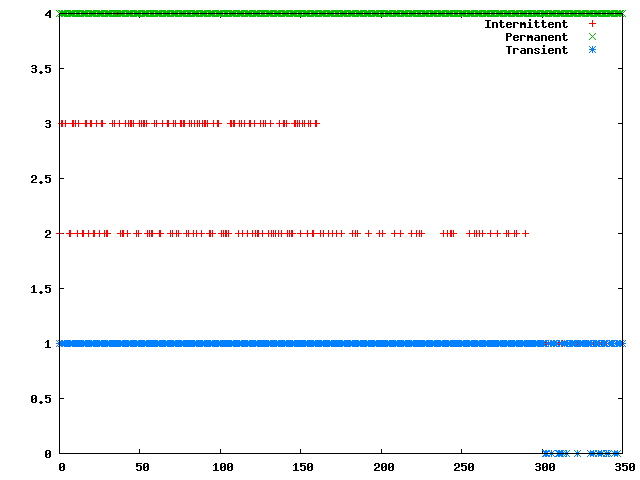
\includegraphics[scale=0.35]{figures/epsilonp45k.png}
    \caption{Plot of $\epsilon$ for p45k}
    \label{fig:epsilonp45k}
  \end{center}
\end{figure}

\subsection{Resemblance of erroneous output patterns}
Resemblance of erroneous output patterns is defined in terms of hamming distance between a set of erroneous output patterns obtained during multiple test runs, for the same input test pattern in a test set. \emph{Hamming Distance} of a set is evaluated as maximum of number of positions in which output patterns differ, pairwise. It is denoted using notation $\delta_H$, subscript $H$ stands for \enquote{horizontal}, denoting the orientation of calculation of the hamming distance. If all output patterns for an input test pattern are correct then the hamming distance and hence the value of $\delta_H$ would be zero.

\begin{figure}[h]
  \begin{center}
    \captionsetup{justification=centering}
    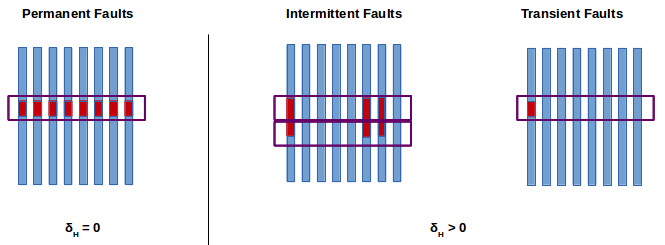
\includegraphics[scale=1.00]{figures/deltah.png}
    \caption{Expected behavior of $\delta_H$ for different faults}
    \label{fig:deltah}
  \end{center}
\end{figure}

Algorithm~\ref{alg:deltah} explains extraction of $\delta_H$. It takes the expected and actual output patterns as inputs. It then checks if any of output pattern is faulty, to save some computational efforts. If  any of output pattern is faulty, it calculates value of $\delta_H$ and stores it in array against corresponding index of input pattern. Final value of $\delta_H$ is maximum value of $\delta_H$ in this array. 

\begin{algorithm}[H]
  \caption{Algorithm to evaluate $\delta_H$}
  \label{alg:deltah}
  \begin{algorithmic}
 \Procedure{ComputeDeltaH}{Expected output pattern array (EX),Observed output pattern array for all test runs (OP)}
 \State $\delta_H$[size(EX)] $\leftarrow$ 0\;
 \State Index $\leftarrow$ 0\;
 \While{Index $<$ size(EX)}
  \If{EX[Index] $\neq$ any pattern of OP[Index][]}
   \State $\delta_H$[Index] $\leftarrow$ \Call{HammingDistance}{OP[Index][]}\;
  \Else
   \State $\delta_H$[Index] $\leftarrow$ 0\;
  \EndIf
  \State Index++\;
 \EndWhile
 \State$\delta_H$ $\leftarrow$ max($\delta_H$[])\;
 \State \Return $\delta_H$\;
 \EndProcedure
 \end{algorithmic}
\end{algorithm}

Figure~\ref{fig:deltah} shows expected behavior of $\delta_H$ for different fault types. Permanent faults repeat with same faulty output pattern and value of $\delta_H$ is expected to be zero. Intermittent faults, even though fail with same faulty output, are not repeatable and hence are expected to have a $\delta_H$ value other than zero. Transient fail randomly at random output locations and hence are expected to have higher $\delta_H$ value. Figure~\ref{fig:deltahp45k} shows actual values of $\delta_H$ for a simple circuit (p45k).

\begin{figure}[h]
  \begin{center}
    \captionsetup{justification=centering}
    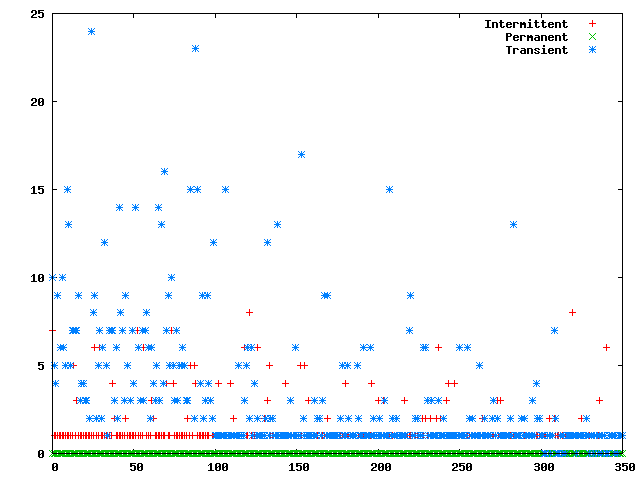
\includegraphics[scale=0.35]{figures/deltahp45k.png}
    \caption{Plot of $\delta_H$ for p45k}
    \label{fig:deltahp45k}
  \end{center}
\end{figure}

\subsection{Resemblance of erroneous primary outputs}
Resemblance of erroneous primary outputs is defined as hamming distance between primary output locations, that showed a faulty behavior at least once for a respective test run. This quantity is denoted by $\delta_V$, subscript $V$ denoting \emph{vertical} collapsing of all faulty primary outputs for a test run, before evaluating hamming distance.

Algorithm~\ref{alg:deltav} explains extraction of $\delta_V$. It takes expected output pattern and actual output patterns as inputs. It then marks the pins which showed faulty behavior at least once in a single test run of complete pattern set, as dirty. Hence number of elements in array of $\delta_V$ equals number of test runs. The final value of $\delta_V$ is hamming distance of $\delta_V$ array.

\begin{algorithm}[H]
  \caption{Algorithm to evaluate $\delta_V$}
  \label{alg:deltav}
  \begin{algorithmic}
 \Procedure{ComputeDeltaV}{Expected output pattern array (EX),Observed output pattern array for all test runs (OP)}
 \State $\delta_V$[TotalRuns] $\leftarrow$ 0\;
 \State CurrentRun $\leftarrow$ 0\;
 \While{CurrentRun $<$ TotalRuns}
  \State Index $\leftarrow$ 0\;
  \While{Index $<$ size(EX)}
	\State ExpectedOutput $\leftarrow$ EX[Index]\;
	\State ActualOutput $\leftarrow$ OP[Index][CurrentRun]\;
   \State Iterator $\leftarrow$ 0\;
	\While{Iterator $<$ length(ExpectedOutput)}
		\If{ExpectedOutput.CharAt(Iterator) $\neq$ ActualOutput.CharAt(Iterator)}
		 \State $\delta_V$[CurrentRun].CharAt(Iterator) $\leftarrow$ 1\;
		\Else
		 \State $\delta_V$[CurrentRun].CharAt(Iterator) $\leftarrow$ 0\;
		\EndIf
		\State Iterator++\;
		\EndWhile
	\State Index++\;
  \EndWhile
 \State CurrentRun++\;
 \EndWhile
 \State $\delta_V$ $\leftarrow$ \Call{HammingDistance}{$\delta_V$[]}\;
 \State \Return $\delta_V$\;
 \EndProcedure
 \end{algorithmic}
\end{algorithm}

It is expected that value of $\delta_V$ is low in case of permanent and intermittent faults, as these faults manifest into failures at fixed set of output pins. In contrast, transient faults do not have a fixed set of outputs that it affects,resulting in high expected value of $\delta_V$.  Figure~\ref{fig:deltavp45k} shows actual values of $\delta_V$ for a simple circuit (p45k).

\begin{figure}[h]
  \begin{center}
    \captionsetup{justification=centering}
    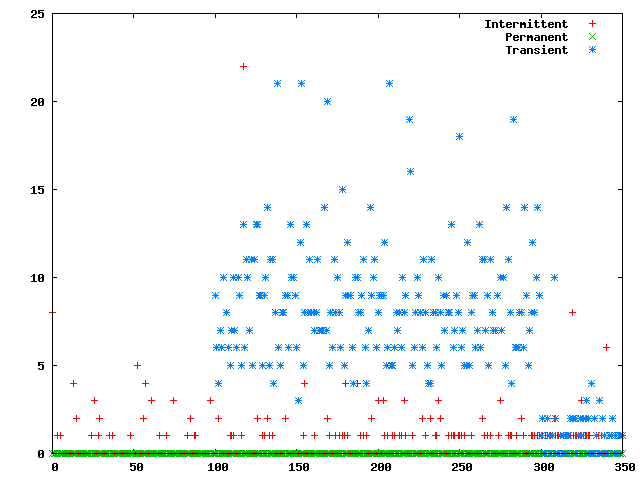
\includegraphics[scale=0.35]{figures/deltavp45k.png}
    \caption{Plot of $\delta_V$ for p45k}
    \label{fig:deltavp45k}
  \end{center}
\end{figure}

\subsection{Diagnostic features}
Diagnostic features from section~\ref{sec:secfd} are also considered as features for learning algorithm. Diagnostic data also provides information about fault present in circuit. A short summery of fault models and observed behavior for diagnostic parameters is summarized in table~\ref{tab:diagparam}. This table is taken from original work by Holst \emph{et.al.} \cite{Holst2009}.

{%
\newcommand{\mc}[3]{\multicolumn{#1}{#2}{#3}}
\begin{table}[h]
    \label{tab:diagparam}
	\captionsetup{justification=centering}
    \begin{tabular}{lccc}
	\hline
    \mc{1}{c}{\textbf{Fault Model}}        & \mc{1}{c}{\textbf{$\iota_T$}} & \mc{1}{c}{\textbf{$\tau_T$}} & \mc{1}{c}{\textbf{$\gamma_t$}} \\
	\hline
    Single stuck-at                       & 0      & 0     & 0       \\
    Stuck-at, multiple fault sites        & 0      &  > 0  & 0       \\
    Single conditional stuck-at           &  > 0   & 0     & 0       \\
    Cond. stuck-at, multiple fault sites  &  > 0   &  > 0  & 0       \\
    Delay fault, i.e. long paths fail     &  > 0   & 0     & > 0     \\ 
	\hline
    \end{tabular}
    \caption {Fault evidence compared with fault models}
\end{table}
}%

In this work it is assumed that at most only a single intermittent or permanent fault is active in the circuit with or without some transient noise (Reference to assumptions section in chap 5). Most of permanent faults can be modeled as single stuck-at, single conditional stuck-at or a delay faults. Transient faults can be modeled as conditional stuck-at faults, at multiple fault sites as the do not have a fixed location on chip and some deterministic probability function can be used as trigging condition. Similarly intermittent faults can be modeled as single conditional stuck-at faults. Hence combination of values of parameters can be used to deduce which type of fault might exist on the chip.

Furthermore, the standard deviation of evidence parameters is expected to be around zero for permanent faults, as once they are detected then they always be detected using same test pattern set. Hence as standard deviations of evidence based features convey some information about fault class, they also considered as features for learning. Figure~\ref{fig:sdevidance} shows actual values of standard deviation of evidence based features for a simple circuit (p45k).

\begin{figure}
        \centering
			\captionsetup{justification=centering}
        \begin{subfigure}[h]{0.45\linewidth}
                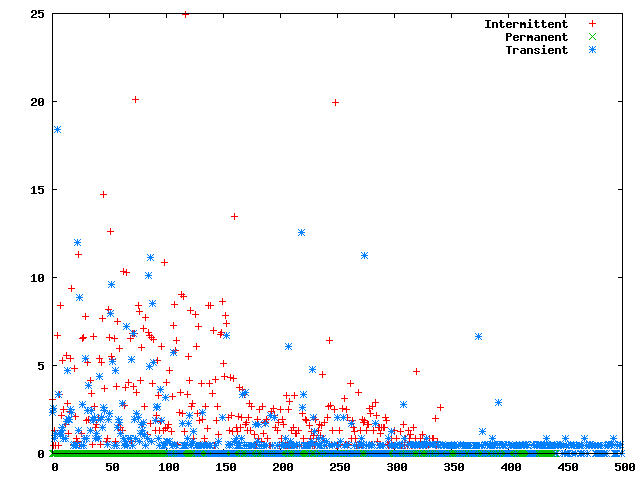
\includegraphics[scale=0.25]{figures/sdsigmap45k.png}
                \caption{Sigma ($\sigma$)}
        \end{subfigure}
        \begin{subfigure}[h]{0.45\linewidth}
                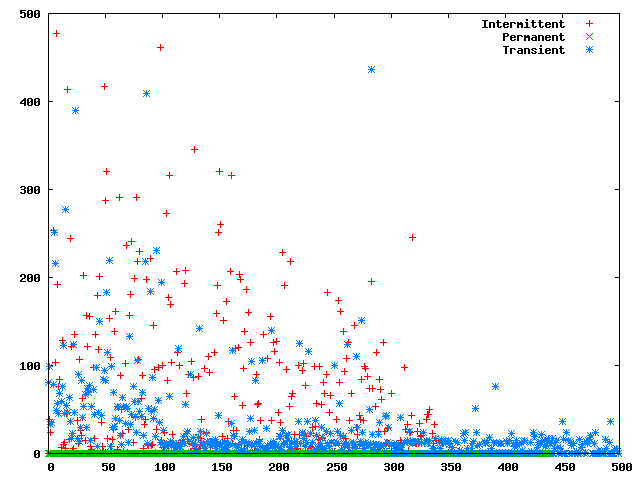
\includegraphics[scale=0.25]{figures/sdiotap45k.png}
                \caption{Iota ($\iota$)}
        \end{subfigure}
			\begin{subfigure}[h]{0.45\linewidth}
                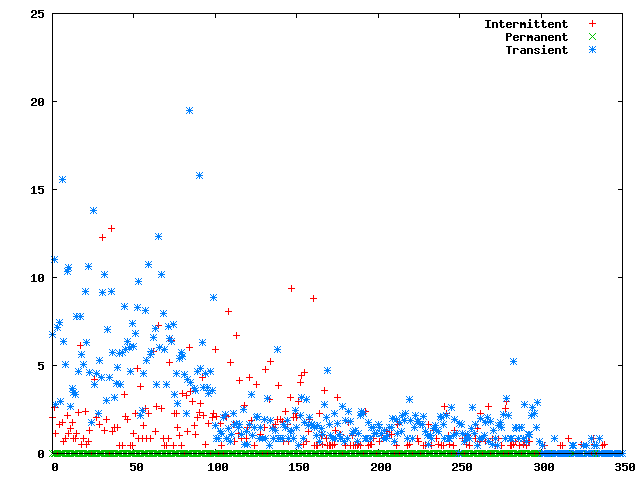
\includegraphics[scale=0.25]{figures/sdtaup45k.png}
                \caption{Tau ($\tau$)}
        \end{subfigure}
        \caption{Standard deviations for evidence-based parameters for p45k}
        \label{fig:sdevidance} 
\end{figure}

Table~\ref{tab:features} summarizes the selected features.
{%
\newcommand{\mc}[3]{\multicolumn{#1}{#2}{#3}}
\label{tab:features}
\captionsetup{justification=centering}
\begin{table}[h]
\begin{tabular}{lll}
\hline
\mc{1}{c}{\textbf{Category}}        & \mc{1}{c}{\textbf{Feature}}       & \mc{1}{c}{\textbf{Symbol}}\\
\hline
\multirow{3}{*}{Non-evidence based features} & Reproducible of fault                    & $\sigma$\\
                                             & Resemblance of erroneous output patterns  & $\delta_H$\\
                                             & Resemblance of erroneous primary outputs   & $\delta_V$\\
\hline
\multirow{8}{*}{Evidence based features}     & Maximum $\sigma$ among all test runs          & $\sigma$\\
                                             & $\iota$ corresponding to maximum $\sigma$  & $\iota$                             \\
                                             & $\tau$ corresponding to maximum $\sigma$   & $\tau$ \\
                                             & $\gamma$ corresponding to maximum $\sigma$ & $\gamma$ \\
                                             & Standard deviation of $\sigma$             & SD($\sigma$)\\
                                             & Standard deviation of $\iota$              & SD($\iota$)\\
                                             & Standard deviation of $\tau$               & SD($\tau$)\\
                                             & Standard deviation of $\gamma$             & SD($\gamma$)\\
\hline
\end{tabular}
\caption{Summary of selected features}
\end{table}
}%

\section{Selection of machine learning algorithm for fault classification}
\label{sec:selml}

There are variety of machine learning algorithms available, and some of the important ones were surveyed in chapter~\ref{chap:chapter3}. The accuracy of machine learning classifier depends mainly on the complexity of the feature space and actual training data at hand. Now that the feature set known, selection of classifier is done with respect to the following factors:

\begin{description}
  \item[Feature set] The feature set is not statistically independent, an important consideration as it violates the prerequisite for Bayes classifier. It can be seen from plots presented in section~\ref{sec:secfs}, that the feature space has high variance and it is not linearly separable, thus it is not practical to come up with rules to classify faults and hence, the performance of decision trees can be expected to be on the lower side. Also, as the feature space is highly complex, polynomial functions in MLPs might not be sufficient to create an acceptable hypothesis, can take long time to train using higher order polynomials and can result overfitting the training data. SVMs, on the other hand can handle kernel functions and can be expected to create a complex hypothesis, as required in our case.

  \item[Sample population] Size of our training data set is limited, as it needs to be generated on a simulator(refer section~\ref{sec:gsp}). Neural networks and decision trees are known to work well with large training sets \cite{DeFries2000,Tanwani2009}. On the other hand, SVMs are shown to be effective with limited size of data sets\cite{Koggalage2004}. The sample population that we have used is not created according to the probabilities of fault occurrence in real world data. It is also not possible to do so otherwise because of two main reasons, first, it is hard to get hands on actual production numbers for evaluation of results, as those numbers a closely guarded company secrets. And second, in actual application scenario, it is hard to predict probabilities of fault occurrence. This makes impossible to set set up prior probabilities required for Bayes classifier.
\end{description}

With this, it becomes clear that SVM can be used as classifier of choice as:
\begin{itemize}
  \item SVMs can work well with small and medium size data sets, with relatively high accuracy \cite{Koggalage2004, Matlab2014}.
  \item They can handle n-dimensional feature spaces.
  \item By construction, they can handle complex of feature spaces with use of kernel functions.
  \item Once trained, they are fast to classify data .
\end{itemize}
%Die Angabe des schlauen Spruchs auf diesem Wege funtioniert nur,
%wenn keine Änderung des Kapitels mittels den in preambel/chapterheads.tex
%vorgeschlagenen Möglichkeiten durchgeführt wurde.
\chapter{Experimental Setup}
\label{chap:chapter5}
%\vspace{-3cm}
%\vspace{2cm}
With the selection and their extraction and SVM, as the selected machine learning algorithm explained in earlier chapter, this chapter explains the experimental setup. This chapter focuses on two topics - first part being the assumptions for the test setup and the configuration of the sample population as well as the method used to generate the sample population, explained in the section~\ref{sec:gsp}. Second part, section~\ref{sec:libsvm} describes the SVM library used for training and classification of faults and its interface with generated samplae population.
\section{Generation of sample population}
\label{sec:gsp}
Sample population is required to train and cross-validate the machine learning based classifier (hereon referred simply as \emph{classifier}). A separate set of data is used to test the accuracy of the classifier.
\subsection{Assumptions}
\label{sec:gsp:assumptions}
Following are the assumptions while generating the sample population and test data:
\begin{enumerate}
  \item It is assumed that the chips to be classified have displayed faulty behavior and hence were rejected in earlier test.
  \item The chips under consideration are either:
		  \begin{enumerate}
    		\item Healthy chips with transient noise or
    		\item Affected by a single permanent or intermittent fault, with or without transient noise.
 		 \end{enumerate}
	\item Number of simulation runs to extract features is fixed at 4. This value is set experimentally. 
\end{enumerate}

\subsection{Configuration}
\label{sec:gsp:configuration}
For the purpose of running experiments uniformly on different circuit types, a sample population and a test set for each of circuit types is created with following configuration:
\begin{enumerate}
  \item A sample population consist of 2500 ($\pm$ 75) of labeled examples. The tolerance of $\pm$ 75 is set as the permanent or intermittent fault instances which did not show any faulty behavior at POs at all were removed.
  \item The sample population is equally divided into following five fault categories:
		\begin{enumerate}
    		\item Permanent faults with label \texttt{P}.
    		\item Permanent faults along with transient noise (fault rate = 0.001) with label \texttt{P}.
			\item Intermittent faults (fault rate = 0.1, 0.01 0.001) with label \texttt{I}.
    		\item Intermittent faults (fault rate = 0.1, 0.01, 0.001) along with transient noise (fault rate = 0.001) with label \texttt{I}.
			\item Transient faults (fault rate = 0.01, 0.001, 0.0001) with label \texttt{T}.
		\item Permanent faults are modeled using stuck-at, wired or delay faults, Intemittents are modeled using high frequency power droop, and transient faults are modeled as conditional stuck-at faults at random locations, triggered using deterministic fault rate.
 		 \end{enumerate}
  \item Test data has 250 ($\pm$ 15) labeled examples, with same configuration as that for sample population.
\end{enumerate}

\subsection{Implementation}

Sample population is generated as shown in figure~\ref{fig:sampopl} using a simulation framework called Adaptive Diagnosis of Arbitrary Manifold Artifacts (ADAMA). ADAMA can be used for logic simulation with error injection. Logical representation of a circuit at gate level and test pattern set are the required inputs for simulation using ADAMA. A fault description can be provided optionally to inject a fault and analyze its behavior. ADAMA supports all of the fault models that have been considered under configuration in section~\ref{sec:gsp:configuration}.

\begin{figure}[h]
  \begin{center}
    \captionsetup{justification=centering}
    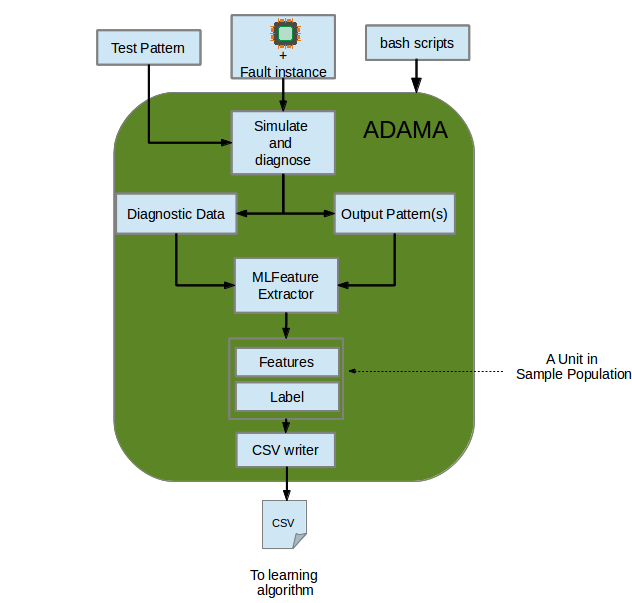
\includegraphics[scale=0.45]{figures/sampopl.png}
    \caption{Generation of sample population using \texttt{spgen}}
    \label{fig:sampopl}
  \end{center}
\end{figure}

For experiments, ADAMA framework has been extended by adding a task to generate sample population, called \texttt{spgen}.\texttt{spgen} takes fault description, circuit description and test pattern set as inputs along with number of simulations runs (\texttt{simruns}) to be performed for feature extraction. It then runs simulation and diagnosis \texttt{simruns} times and passes it on to the object of class \texttt{MLFeatureExtractor}, which encompasses all of the procedures for feature extraction described in section~\ref{sec:secfs} of previous chapter. Once complete simulation is over, it writes the features and its label in a CSV file.

Shell scripts are used to invoke instances of ADAMA and inject fault instances of permanent, transient and intermittent faults. The process to do the same is described below:

\begin{description}
  \item[Permanent Faults] A task in ADAMA called \texttt{fsample} is used to generate fault descriptions for permanent faults. Script first runs task \texttt{fsample} and puts all fault descriptions in a file, and then parses it line-by-line to invoke an instance of ADAMA with task \texttt{spgen}. It then uses same fault descriptions and adds a transient fault instance to generate transient noise and runs the complete process again, while logging seed values used to generate transients. After generation of features is done, it scans through the feature file of permanent faults without transient noise and scans for fault instances which did not result in failure at POs and removes corresponding features, fault descriptions and corresponding items in feature file for permanent faults with transient noise.

  \item[Intermittent faults] Script first generates intermittent fault descriptions with random seed values for location and fault activation and store them into a file. It then invokes \texttt{spgen} using ADAMA and simulates these fault instances first without and then with transient noise, while logging all seed values and corresponding fault rates. The fault descriptions and and corresponding examples in feature files of intermittent faults and intermittent faults with transient noise are removed, where intermittent fault as not active at least for one simulation round.

  \item[Transient faults] Script takes circuit description and passes it, along with a transient fault instance with defined fault rate and a randomly generated seed value to \texttt{spgen} in ADAMA. It also logs seed values and corresponding fault rates used for generation of transient fault instances.
\end{description}

\section{Library for SVM based classification - \texttt{LIBSVM}}
\label{sec:libsvm}
\texttt{LIBSVM} \cite{Chang2011} is a popular SVM library, used in variety of applications. It supports linear, polynomial, radial and sigmoid kernel functions and also supports custom user kernels. For experiments, all of the available kernels in the tool have been used, to find out accuracy levels for each of them. It is coded in C++ and Java and it is available as open-source software available for free use under modified BSD license. It supports multi-class classification using multiple binary classifiers. \texttt{LIBSVM} comes with scripts to train the tool and to find optimal parameters for classification.

\subsection{Training}

\begin{figure}[h]
  \begin{center}
    \captionsetup{justification=centering}
    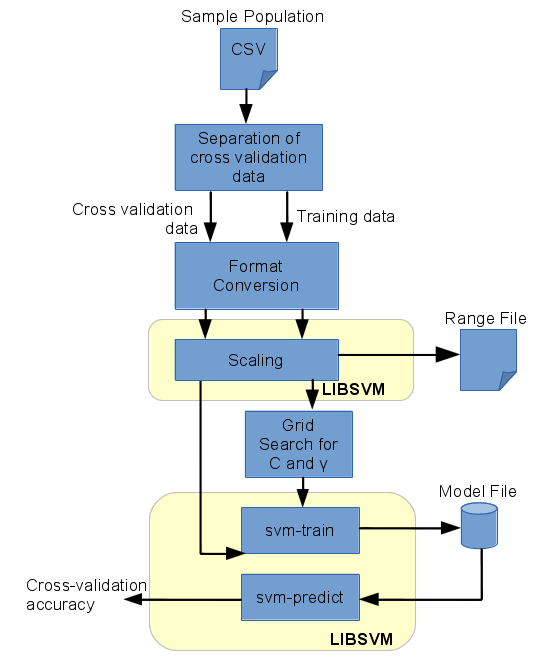
\includegraphics[scale=0.75]{figures/libsvmtrain.png}
    \caption{Steps to train SVM using \texttt{LIBSVM}}
    \label{fig:libsvmtrain}
  \end{center}
\end{figure}

Sequence of steps followed to train SVM, as shown in figure~\ref{fig:libsvmtrain} is as follows:
\begin{description}
   \item[Format conversion] \texttt{LIBSVM} requires input in \emph{sparse} format. A utility function \texttt{convert} provided by authors of \texttt{LIBSVM} has been extended to be compatible with the CSV format output of \texttt{spgen}.

  \item[Scaling] \texttt{svm-scale} executable file in \texttt{LIBSVM} provides functionallity to scale the training data to user specified input range. Documentation of \texttt{LIBSVM} \cite{Hsu2003} suggest use of range [0,1] for the data containing zero values for some of feaures, as in our case. The scaling parameters are stored in a \emph{range file}, which is later used to scale features of future examples or test data.
  
  \item[Grid search for C and $\gamma$] \texttt{LIBSVM} provides a script to find suitable values of C and $\gamma$. The grid search algorithm uses $v$-fold cross-validation (CV), meaning that the data is divided into $v$ subsets and one subset is tested against classifier trained with rest of $v-1$ subsets, iteratively until complete training set is covered \cite{Hsu2003}.  This results in the training data being tested once completely, and corresponding accuracy is called as \emph{cross-validation accuracy}. The algorithm then tries various pairs of C and $\gamma$ to find a pair with the highest CV accuracy. This script internally uses \texttt{svm-train} for modeling classifiers, when it calculates CV accuracy, hence the kernel type for training needs to be specified. This script was extended to take kernel type as input.
 
 \item[Training] \texttt{svm-train} executable file in \texttt{LIBSVM} is used for training SVM. It tries to solve the minimization problem (refer section~\ref{mltypes:svm}) to find out best fitting model for the SVM. Kernel to be used for training needs to be provided as input at this stage also. It outputs a \emph{model file} to be used for prediction of future examples.
\end{description}

\subsection{Classification}

Steps to classify data using already trained SVM is shown in figure~\ref{fig:libsvmpredict}. A short description of the these is noted below:

\begin{figure}[h]
  \begin{center}
    \captionsetup{justification=centering}
    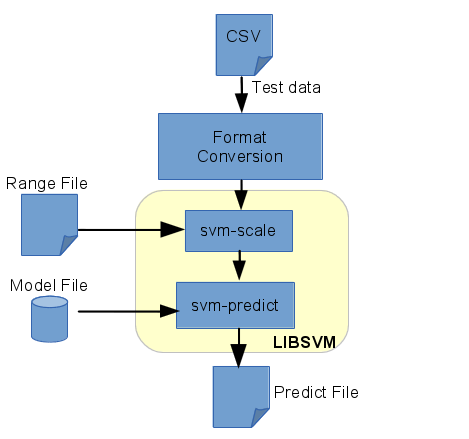
\includegraphics[scale=0.75]{figures/libsvmpredict.png}
    \caption{Steps for classification of test data with SVM using \texttt{LIBSVM}}
    \label{fig:libsvmpredict}
  \end{center}
\end{figure}

\begin{description}

   \item[Format conversion] Using the same tool used for format conversion of training data, format of test data is also converted to sparse format.

  \item[Scaling] The test data is scaled using \texttt{svm-scale}. The range file generated while scaling the training data is used in this step to scale the test data.
  
  \item[Prediction] \texttt{svm-predict} tool provided with \texttt{LIBSVM} is used to predict the test data. \texttt{svm-predict} needs model file generated during training as input and it outputs \emph{predict file} with predicated labels of the test data. This file is further processed using scripts for evaluation of accuracy levels of different fault classes.
  
\end{description}

%Die Angabe des schlauen Spruchs auf diesem Wege funtioniert nur,
%wenn keine Änderung des Kapitels mittels den in preambel/chapterheads.tex
%vorgeschlagenen Möglichkeiten durchgeführt wurde.
\chapter{Evaluation of results}
\label{chap:chapter6}
%\vspace{-3cm}
%\vspace{2cm}
This chapter presents results of classification using experimental setup described in chapter~\ref{chap:chapter6}. The term \emph{Classification accuracy} of a class used in chapter is defined as,

\[ \begin{array}{ll} accuracy(r_i) = \frac{\mbox{Samples correctly predicted as $r_i$}}
								{\mbox{Total samples with label $r_i$}}
							\times 100 & 
							\forall \,r_i \in \{\mbox{\texttt{P,I,T}}\} 
	\end{array}\]

Where, $r$ is the label of test sample $x=\{\boldsymbol{x},r\}$.

In the presented evaluation, cross-validation accuracy is also noted for each set of experiments, as this is value of accuracy during self-validation of much larger training set.

In the first part analyzes classification efficiency after grid search for optimal values of $C$ and $\gamma$, but does not consider any other optimization, detailed account of results are presented for each kernel type available in \texttt{LIBSVM}. Second part improvises the first, and results are noted after optimization of so-called \emph{class-weights}. Third part explores two possibilities -that of using one  of using single prediction model for predicting all types of circuits, and second to extrapolating known model to predict new circuit types. The last part tries to evaluate impact on yield and quality of final product after application of suggested method.

\section{Classification of permanent faults}

Consider a special case, where $\epsilon = Test Runs$. In our classification problem this can mean,
\begin{enumerate}
  \item It is a permanent fault.
  \item A rare case of highly repetitive intermittent fault, and can be said to be \enquote{critical}.
  \item An extremely rare transient fault, as it happened at the same location and for same input test pattern, in all of the test runs.
\end{enumerate}

In the other direction, for permanent faults $\epsilon = Test Runs$ holds true, except a rare possibility that transient noise affects all the test patterns, which have resulted in failure at POs, in at least one of test runs. This is also an extremely rare possibility. Hence we assume that, a fault is permanent if and only if $\epsilon = Test Runs$.

If we go back to section~\ref{sec:secfs} and observe the plot for $\epsilon$ in figure~\ref{fig:epsilonp45k}, we can observe our assumption to be fairly accurate. Hence if we do a slight modification in our experimental setup and already remove faults where $\epsilon = Test Runs$, and classify them as permanent faults, we can achieve 100\% permanent fault classification, and we would be left with a binary classification problem between transient and intermittent faults. 

\section{Classification without class-weight optimization}
First set of experiments consist of evaluation of accuracy levels without assigning class weights \emph{i.e.} class-weights are assumed to be \{1,1,1\} for permanent, intermittent and transient faults respectively. The experiments are carried out for variety of circuits ranging from simple p45k to highly complex p295k. The experiments are repeated for each type of kernel provided by \texttt{LIBSVM}. 

This set of experiments consist of two rounds each for each kernel, first one includes permanent faults in sample population, the other one without considering them. A round with permanents is carried out only to evaluate change in accuracy levels of classification.

\subsection{Linear Kernel}
Accuracy of SVM using linear kernel is summarized in table~\ref{tab:linwp} with considering permanent faults in sample population, and the same without considering permanents is summarized in table~\ref{tab:linwop}.
\begin{table}[h]

	\captionsetup{justification=centering}
\begin{tabular}{ccccccc}
\hline
\multicolumn{1}{c}{\multirow{3}{*}{Circuit}} & \multicolumn{6}{c}{Accuracy (\%)}\\ \cline{2-7} 
\multicolumn{1}{c}{}                         & \multicolumn{1}{c}{\multirow{2}{*}{Cross-validation}} & \multicolumn{2}{c}{Permanent} & \multicolumn{2}{c}{Intermittent} & \multicolumn{1}{c}{\multirow{2}{*}{Transient}} \\ \cline{3-6}
                                             &                                                       & w/o noise     & with noise    & w/o noise      & with noise      &                                                \\ \hline
p45k                                         & 90.14                                                 & 87.50         & 87.50         & 77.50          & 64.58           & 93.90                                          \\
p100k                                        & 87.38                                                 & 100           & 100           & 80.95          & 57.14           & 95.91                                          \\
p141k                                        & 83.89                                                 & 98.21         & 98.21         & 61.90          & 57.14           & 100                                            \\
p267k                                        & 85.12                                                 & 100           & 100           & 55.00          & 52.50           & 100                                            \\
p279k                                        & 89.52                                                 & 98.30         & 96.61         & 78.94          & 52.50           & 89.79                                          \\
p295k                                        & 89.84                                                 & 100           & 100           & 81.39          & 65.11           & 100   \\
\hline                                        
\end{tabular}
\caption {Classification accuracy for linear kernel}
\label{tab:linwp}
\end{table}

\begin{table}[h]

	\captionsetup{justification=centering}
\begin{tabular}{ccccc}
\hline
\multirow{3}{*}{Circuit} & \multicolumn{4}{c}{Accuracy (\%)}\\ \cline{2-5} 
                         & \multirow{2}{*}{Cross-validation} & \multicolumn{2}{c}{Intermittent} & \multirow{2}{*}{Transient} \\ \cline{3-4}
                         &                                   & w/o noise      & with noise      &                            \\ \hline
p45k                     & 87.81                             & 72.91          & 70.08           & 97.95                      \\
p100k                    & 81.43                             & 69.05          & 59.52           & 97.96                      \\
p141k                    & 84.13                             & 21.42          & 76.19           & 100                        \\
p267k                    & 77.09                             & 80.00          & 55.00           & 100                        \\
p279k                    & 84.65                             & 78.94          & 52.63           & 91.83                      \\
p295k                    & 89.17                             & 90.69          & 81.39           & 100           \\
\hline            
\end{tabular}
\caption {Classification accuracy for linear kernel, without permanent faults}
\label{tab:linwop}
\end{table}


\subsection{Polynomial Kernel}


\begin{table}[h]

	\captionsetup{justification=centering}
\begin{tabular}{ccccccc}
\hline
\multirow{3}{*}{Circuit} & \multicolumn{6}{c}{Accuracy (\%)}\\ \cline{2-7} 
                         & \multirow{2}{*}{Cross-validation} & \multicolumn{2}{c}{Permanent} & \multicolumn{2}{c}{Intermittent} & \multirow{2}{*}{Transient} \\ \cline{3-6}
                         &                                   & w/o noise     & with noise    & w/o noise      & with noise      &                            \\ \hline
p45k                     & 90.92                             & 87.50         & 89.58         & 68.75          & 70.83           & 83.67                      \\
p100k                    & 89.70                             & 100           & 97.82         & 69.04          & 66.66           & 93.87                      \\
p141k                    & 87.94                             & 100           & 100           & 73.80          & 71.42           & 95.00                      \\
p267k                    & 87.34                             & 100           & 96.55         & 82.50          & 60.00           & 85.71                      \\
p279k                    & 91.42                             & 98.30         & 96.55         & 81.57          & 73.68           & 91.83                      \\
p295k                    & 90.78                             & 100           & 98.21         & 76.09          & 72.09           & 95.91      \\
\hline                                                     
\end{tabular}
\caption {Classification accuracy for polynomial kernel}
\label{tab:polywp}
\end{table}

\begin{table}[h]

	\captionsetup{justification=centering}
\begin{tabular}{ccccc}
\hline
\multirow{3}{*}{Circuit} & \multicolumn{4}{c}{Accuracy (\%)}\\ \cline{2-5} 
                         & \multirow{2}{*}{Cross-validation} & \multicolumn{2}{c}{Intermittent} & \multirow{2}{*}{Transient} \\ \cline{3-4}
                         &                                   & w/o noise      & with noise      &                            \\ \hline
p45k                     & 87.81                             & 81.25          & 72.91           & 87.76                      \\
p100k                    & 85.00                             & 78.57          & 66.66           & 89.79                      \\
p141k                    & 85.57                             & 80.95          & 76.19           & 100                        \\
p267k                    & 81.38                             & 82.50          & 72.50           & 93.87                      \\
p279k                    & 85.57                             & 78.94          & 73.68           & 93.87                      \\
p295k                    & 92.28                             & 93.02          & 86.04           & 93.87                      \\
\hline
\end{tabular}
\caption {Classification accuracy for polynomial kernel, without permanent faults}
\label{tab:polywop}
\end{table}



\subsection{RBF Kernel}
\begin{table}[h]

	\captionsetup{justification=centering}
\begin{tabular}{ccccccc}
\hline
\multirow{3}{*}{Circuit} & \multicolumn{6}{c}{Accuracy (\%)}\\ \cline{2-7} 
                         & \multirow{2}{*}{Cross-validation} & \multicolumn{2}{c}{Permanent} & \multicolumn{2}{c}{Intermittent} & \multirow{2}{*}{Transient} \\ \cline{3-6}
                         &                                   & w/o noise     & with noise    & w/o noise      & with noise      &                            \\ \hline
p45k                     & 91.21                             & 100           & 100           & 66.66          & 64.58           & 91.83                      \\
p100k                    & 87.36                             & 100           & 100           & 64.28          & 61.94           & 93.87                      \\
p141k                    & 88.63                             & 100           & 100           & 73.80          & 71.42           & 93.87                      \\
p267k                    & 87.27                             & 100           & 98.27         & 80.00          & 72.50           & 93.87                      \\
p279k                    & 89.52                             & 98.30         & 96.55         & 78.94          & 71.05           & 93.87                      \\
p295k                    & 91.00                             & 100           & 100           & 79.06          & 74.41           & 95.91                     \\
\hline                                                     
\end{tabular}
\caption {Classification accuracy for RBF kernel}
\label{tab:rbfwp}
\end{table}

\begin{table}[h]

	\captionsetup{justification=centering}
\begin{tabular}{ccccc}
\hline
\multirow{3}{*}{Circuit} & \multicolumn{4}{c}{Accuracy (\%)}                                                                 \\ \cline{2-5} 
                         & \multirow{2}{*}{Cross-validation} & \multicolumn{2}{c}{Intermittent} & \multirow{2}{*}{Transient} \\ \cline{3-4}
                         &                                   & w/o noise      & with noise      &                            \\ \hline
p45k                     & 87.56                             & 77.08          & 70.83           & 91.83                      \\
p100k                    & 83.33                             & 78.57          & 64.28           & 89.79                      \\
p141k                    & 86.53                             & 83.33          & 80.95           & 100                        \\
p267k                    & 80.19                             & 82.50          & 70.00           & 95.91                      \\
p279k                    & 85.64                             & 78.92          & 76.31           & 95.91                      \\
p295k                    & 85.64                             & 78.92          & 76.31           & 95.91  						  \\
\hline
\end{tabular}
\caption {Classification accuracy for RBF kernel, without permanent faults}
\label{tab:rbfwop}
\end{table}

\subsection{Sigmoid Kernel}

\begin{table}[h]

	\captionsetup{justification=centering}
\begin{tabular}{ccccccc}
\hline
\multirow{3}{*}{Circuit} & \multicolumn{6}{c}{Accuracy (\%)}                                                                                                 \\ \cline{2-7} 
                         & \multirow{2}{*}{Cross-validation} & \multicolumn{2}{c}{Permanent} & \multicolumn{2}{c}{Intermittent} & \multirow{2}{*}{Transient} \\ \cline{3-6}
                         &                                   & w/o noise     & with noise    & w/o noise      & with noise      &                            \\ \hline
p45k                     & 89.55                             & 87.50         & 87.50         & 77.08          & 60.41           & 95.91                      \\
p100k                    & 85.08                             & 100           & 100           & 95.23          & 52.38           & 71.42                      \\
p141k                    & 84.17                             & 100           & 100           & 57.14          & 57.14           & 100                        \\
p267k                    & 82.46                             & 100           & 98.27         & 42.50          & 42.50           & 100                        \\
p279k                    & 89.29                             & 98.30         & 96.55         & 81.57          & 52.63           & 87.76                      \\
p295k                    & 85.09                             & 98.21         & 98.21         & 69.76          & 65.11           & 100                       \\
\hline                                                     
\end{tabular}
\caption {Classification accuracy for sigmoid kernel}
\label{tab:sigwp}
\end{table}


\begin{table}[h]

	\captionsetup{justification=centering}
\begin{tabular}{ccccc}
\hline
\multirow{3}{*}{Circuit} & \multicolumn{4}{c}{Accuracy (\%)}                                                                 \\ \cline{2-5} 
                         & \multirow{2}{*}{Cross-validation} & \multicolumn{2}{c}{Intermittent} & \multirow{2}{*}{Transient} \\ \cline{3-4}
                         &                                   & w/o noise      & with noise      &                            \\ \hline
p45k                     & 84.46                             & 68.75          & 60.41           & 100                        \\
p100k                    & 80.00                             & 81.39          & 52.38           & 100                        \\
p141k                    & 80.04                             & 78.57          & 73.80           & 100                        \\
p267k                    & 75.17                             & 75.00          & 55.00           & 100                        \\
p279k                    & 83.41                             & 81.57          & 52.63           & 91.83                      \\
p295k                    & 92.16                             & 93.02          & 86.04           & 91.83                     \\
\hline
\end{tabular}
\caption {Classification accuracy for sigmoid kernel, without permanent faults}
\label{tab:sigwop}
\end{table}

\subsection{Analysis of intermittent fault classification}
\section{With class-weight optimization}
\section{Other possibilities}
\subsection{Using single training set for prediction}
\subsection{Using known model to extrapolate results}
\section{Impact of yield and quality of final product}

%Die Angabe des schlauen Spruchs auf diesem Wege funtioniert nur,
%wenn keine Änderung des Kapitels mittels den in preambel/chapterheads.tex
%vorgeschlagenen Möglichkeiten durchgeführt wurde.
\chapter{Conclusion and Future Work}
\label{chap:chapter7}
%\vspace{-3cm}
%\vspace{2cm}
\section{Conclusion}

This thesis presented a possibility of using SVM based machine learning approach for fault classification of semiconductor chips. The chips tested showed moderate to high overall accuracy levels for fault classification. Classification of permanent faults showed no significant issues as they are repeatable and their failures are localized to a set of primary outputs. Separating intermittent faults, when their fault activation rates are in lower range and same as those for transient faults, presents a significant challenge as their fault behavior is similar to each other. However, the results show that intermittent faults, at higher fault activation rates are upto 100\% separable from transient faults, even in presence of background noise.


Different kernels were used for SVM and it can be concluded that, selection of kernel primarily depends on the nature of feature space of the subject sample population. High cross-validation accuracy is a good indicator for accuracy and should be used for selection of kernel. However, too-high cross-validation accuracy values might indicate that kernel is overfitting, and it should be then tested with a separate test dataset, and this accuracy should also be considered for kernel selection. Also from the background research for this thesis, it is clear that selection of features plays a crucial role in efficiency, irrespective of chosen algorithm and kernel. A well-balanced dataset, containing equal number of positive and negative examples, is also important in determining performance of the SVM. The imbalance in sample population can somewhat be remedied using class-weights.

A set of experiments was also carried out to assess a possibility of using sample population from one known circuit type, which showed good accuracy levels, to classify faults on unknown circuit types. The experiments show that, this is indeed possible and the accuracy levels were were comparable to, or even better in some cases as compared to those obtained for the same circuits using their own sample population. In a different experiment,  a universal training dataset was also constructed from all known circuit types and result obtained were comparable to those from individual training datasets.

This thesis also proposes a solution were user can optimize fault classification for yield or for quality. In a practical situation where user wants to focus more yield of product and not so much on quality, he can make use of class weights to bias the algorithm to reject chips which showed permanent faults and only severe intermittent faults. On the other hand, when user wishes to focus more on quality, he can choose to add higher weight for intermittent faults, and algorithm will reject all permanents and most of intermittents.

Going back, the motivation of this thesis was to separate critical fault from non-critical ones, to improve yield. The criticality of a fault is an abstract concept and its definition varies as per the application domain of the product. With use of class weights, user should be able to adjust the yield-quality trade-off.

To conclude, machine learning is presented as a feasible option for fault classification. This approach does not require expert knowledge, except during feature selection phase, as once feature selection is done, same features can be used for classification of faults on different circuit types, a certain advantage, unlike rule-based classification approaches where threshold values need to be adjusted by experts for every individual product and technology. Another benefit is that, once training data is ready, machine learning is automated and can be used as a black-box approach to classification. Moreover, the existing classification model can be made adaptive by importing sample populations for new circuit types, making machine learning highly adaptive. 

\section{Future work}

This works presents a preliminary analysis of using SVM as classifier. One of the reasons for choosing SVM for classification, is its strong mathematical foundations \cite{Vapnik1995, Ben-Hur2010} and ability to use multiple kernels for classification. A further analysis is possible using different kernels or algorithms for classification. Classification accuracy has further optimization potential, with use of additional features than those suggested in this work.

The experiments carried out used different circuit types. Results suggested that using a universal model for classification is possible. It might also be possible that, this approach can also work for same circuit types at different technology node. A more elaborate analysis is required to verify the same.

The experiments were carried out using number of $TestRuns = 4$. This figure was set experimentally, to facilitate observability of transient and intermittent failures. Work can be done to ensure practicability of the approach by reducing this number. The sample population was generated by extending simulation framework \texttt{ADAMA}, using fault models already available in the framework. To make approach more precise, additional fault models can be added to generate sample population. A practical solution can also be to use actual manufacturing data from industries, which would be able to replicate more practical failure rates.



%%Die Angabe des schlauen Spruchs auf diesem Wege funtioniert nur,
%wenn keine Änderung des Kapitels mittels den in preambel/chapterheads.tex
%vorgeschlagenen Möglichkeiten durchgeführt wurde.
\setchapterpreamble[u]{%
\dictum[Albert Einstein]{Probleme kann man niemals mit derselben Denkweise lösen, durch die sie entstanden sind.}
}
\chapter{Kapitel zwei}
\label{chap:k2}
%\vspace{-3cm}
%\vspace{2cm}

Hier wird der Hauptteil stehen. Falls mehrere Kapitel gewünscht, entweder mehrmals \texttt{\textbackslash{}chapter} benutzen oder pro Kapitel eine eigene Datei anlegen und \texttt{ausarbeitung.tex} anpassen.

\section{File-Encoding und Unterstützung von Umlauten}
Die Vorlage wurde 2010 auf UTF-8 umgestellt.
TeXnicCenter 1 RC 1 unterstützt \textbf{kein} UTF-8.
Die Alpha-Version soll UTF-8 können, aber es gibt anscheinend Probleme.
Deshalb bitte einen anderen Editor, wie \zB \href{http://texstudio.sourceforge.net/}{TeXstudio} verwenden.

\section{Zitate}
Wörter am besten mittels \texttt{\textbackslash enquote\{...\}} \enquote{einschließen}, dann werden die richtigen Anführungszeichen verwendet.

\section{Mathematische Formeln}
\label{sec:mf}
Mathematische Formeln kann man $so$ setzen. \texttt{symbols-a4.pdf} (zu finden auf \url{http://www.ctan.org/tex-archive/info/symbols/comprehensive/symbols-a4.pdf}) enthält eine Liste der unter LaTeX direkt verfügbaren Symbole. z.\,B.\ $\mathbb{N}$ für die Menge der natürlichen Zahlen. Für eine vollständige Dokumentation für mathematischen Formelsatz sollte die Dokumentation zu \texttt{amsmath}, \url{ftp://ftp.ams.org/pub/tex/doc/amsmath/} gelesen werden.

Folgende Gleichung erhält keine Nummer, da \texttt{\textbackslash equation*} verwendet wurde.
\begin{equation*}
x = y
\end{equation*}

Die Gleichung~\ref{eq:test} erhält eine Nummer:
\begin{equation}
\label{eq:test}
x = y
\end{equation}

Eine ausführliche Anleitung zum Mathematikmodus von LaTeX findet sich in \url{http://www.ctan.org/tex-archive/help/Catalogue/entries/voss-mathmode.html}.

\section{Quellcode}
Listing~\ref{lst:ListingANDlstlisting} zeigt, wie man Programmlistings einbindet.  Mittels \texttt{\textbackslash lstinputlisting} kann man den Inhalt direkt aus Dateien lesen.

%Listing-Umgebung wurde durch \newfloat{Listing} definiert
\begin{Listing}
\begin{lstlisting}
<listing name="second sample">
  <content>not interesting</content>
</listing>
\end{lstlisting}
\caption{lstlisting in einer Listings-Umgebung, damit das Listing durch Balken abgetrennt ist}
\label{lst:ListingANDlstlisting}
\end{Listing}

Quellcode im \lstinline|<listing />| ist auch möglich.

\section{Abbildungen}
Die Abbildungen~\ref{fig:chor1} und~\ref{fig:chor2} sind für das Verständnis dieses Dokuments
wichtig. Im Anhang zeigt Abbildung~\vref{fig:AnhangsChor} erneut die komplette Choreographie.

%Die Parameter in eckigen Klammern sind optionale Parameter - z.B. [htb!]
%htb! bedeutet: "Liebes LaTeX, bitte platziere diese Abbildung zuerst hier ("_h_ere"). Falls das nicht funktioniert, dann bitte oben auf der Seite ("_t_op"). Und falls das nicht geht, bitte unten auf der Seite ("_b_ottom"). Und bitte, bitte bevorzuge hier und oben, auch wenn's net so optimal aussieht ("!")
%Diese sollten nach Möglichkeit NICHT verwendet werden. LaTeX's Algorithmus für das Platzieren der Gleitumgebung ist schon sehr gut!
\begin{figure}
  \begin{center}
    \includegraphics[width=\textwidth]{choreography.pdf}
    \caption{Beispiel-Choreographie}
    \label{fig:chor1}
  \end{center}
\end{figure}

\begin{figure}
  \begin{center}
    \includegraphics[width=.8\textwidth]{choreography.pdf}
    \caption[Beispiel-Choreographie]{Die Beispiel-Choreographie. Nun etwas kleiner, damit \texttt{\textbackslash textwidth} demonstriert wird. Und auch die Verwendung von alternativen Bildunterschriften für das Verzeichnis der Abbildungen. Letzteres ist allerdings nur Bedingt zu empfehlen, denn wer liesst schon so viel Text unter einem Bild? Oder ist es einfach nur Stilsache?}
    \label{fig:chor2}
  \end{center}
\end{figure}

Das SVG in \cref{fig:directSVG} ist direkt eingebunden, während der Text im SVG in \cref{fig:latexSVG} mittels pdflatex gesetzt ist.
\todo{Falls man die Graphiken sehen möchte, muss inkscape im PATH sein und im Tex-Quelltext \texttt{\textbackslash{}iffalse} und \texttt{\textbackslash{}iftrue} auskommentiert sein.}

\iffalse % <-- Das hier wegnehmen, falls inkscape im Pfad ist
\begin{figure}
\centering
\includegraphics{svgexample.svg}
\caption{SVG direkt eingebunden}
\label{fig:directSVG}
\end{figure}

\begin{figure}
\centering
\def\svgwidth{.4\textwidth}
\includesvg{svgexample}
\caption{Text im SVG mittels \LaTeX{} gesetzt}
\label{fig:latexSVG}
\end{figure}
\fi % <-- Das hier wegnehmen, falls inkscape im Pfad ist

\section{Tabellen}
Tabelle~\ref{tab:Ergebnisse} zeigt Ergebnisse.
\begin{table}
  \begin{center}
    \begin{tabular}{ccc}
	\toprule
	\multicolumn{2}{c}{\textbf{zusammengefasst}} & \textbf{Titel} \\ \midrule
	Tabelle & wie & in \\
	\url{tabsatz.pdf}& empfohlen & gesetzt\\
	
	\multirow{2}{*}{Beispiel} & \multicolumn{2}{c}{ein schönes Beispiel}\\
	 & \multicolumn{2}{c}{für die Verwendung von \enquote{multirow}}\\
	\bottomrule
    \end{tabular}
    \caption[Beispieltabelle]{Beispieltabelle -- siehe \url{http://www.ctan.org/tex-archive/info/german/tabsatz/}}
    \label{tab:Ergebnisse}
  \end{center}
\end{table}

\section{Pseudocode}
Algorithmus~\vref{alg:sample} zeigt einen Beispielalgorithmus.
\begin{algorithm} %Die Umgebung nur benutzen, wenn man den Algorithmus ähnlich wie Graphiken von TeX platzieren lassen möchte
\caption{Sample algorithm}
\label{alg:sample}
\begin{algorithmic}
\Procedure{Sample}{$a$,$v_e$}
\State $\mathsf{parentHandled} \gets (a = \mathsf{process}) \lor \mathsf{visited}(a'), (a',c,a) \in \mathsf{HR}$ 
\State \Comment $(a',c'a) \in \mathsf{HR}$ denotes that $a'$ is the parent of $a$
\If{$\mathsf{parentHandled}\,\land(\mathcal{L}_\mathit{in}(a)=\emptyset\,\lor\,\forall l \in \mathcal{L}_\mathit{in}(a): \mathsf{visited}(l))$}
\State $\mathsf{visited}(a) \gets \text{true}$
\State $\mathsf{writes}_\circ(a,v_e) \gets
\begin{cases}
\mathsf{joinLinks}(a,v_e) & \abs{\mathcal{L}_\mathit{in}(a)} > 0\\
\mathsf{writes}_\circ(p,v_e)
& \exists p: (p,c,a) \in \mathsf{HR}\\
(\emptyset, \emptyset, \emptyset, false) & \text{otherwise}
\end{cases}
$
\If{$a\in\mathcal{A}_\mathit{basic}$}
  \State \Call{HandleBasicActivity}{$a$,$v_e$}
\ElsIf{$a\in\mathcal{A}_\mathit{flow}$}
  \State \Call{HandleFlow}{$a$,$v_e$}
\ElsIf{$a = \mathsf{process}$} \Comment Directly handle the contained activity
  \State \Call{HandleActivity}{$a'$,$v_e$}, $(a,\bot,a') \in \mathsf{HR}$
  \State $\mathsf{writes}_\bullet(a) \gets \mathsf{writes}_\bullet(a')$
\EndIf
\ForAll{$l \in \mathcal{L}_\mathit{out}(a)$}
  \State \Call{HandleLink}{$l$,$v_e$}
\EndFor
\EndIf
\EndProcedure
\end{algorithmic}
\end{algorithm}

\clearpage
Und wer einen Algorithmus schreiben möchte, der über mehrere Seiten geht, der kann das nur mit folgendem \textbf{üblen} Hack tun:

{
\begin{minipage}{\textwidth}
\hrule height .8pt width\textwidth
\vskip.15em%\vskip\abovecaptionskip\relax
\%stepcounter{Algorithmus}
%\addcontentsline{alg}{Algorithmus}{\protect\numberline{\theAlgorithmus}{\ignorespaces Description \relax}}
%\noindent\textbf{Algorithmus \theAlgorithmus} Description
\stepcounter{algorithm}
\addcontentsline{alg}{Algorithmus}{\thealgorithm{}\hskip0em Description}
\textbf{Algorithmus \thealgorithm} Description
\vskip.3em%\vskip\belowcaptionskip\relax
\hrule height .5pt width\textwidth
\end{minipage}
code goes here\\
test2\\
\vskip-.9em
\hrule height .5pt width\textwidth
}

\section{Verweise}
Für weit entfernte Abschnitte ist \enquote{varioref} zu empfehlen:
\enquote{Siehe \vref{sec:mf}}.
Das Kommando \texttt{\textbackslash{}vref} funktioniert ähnlich wie \texttt{\textbackslash{}cref} mit dem Unterschied, dass zusätzlich ein Verweis auf die Seite hinzugefügt wird.
\texttt{vref}: \enquote{\vref{sec:diff}}, \texttt{cref}: \enquote{\cref{sec:diff}}, \texttt{ref}: \enquote{\ref{sec:diff}}.

Falls \enquote{varioref} Schwierigkeiten macht, dann kann man stattdessen \enquote{cref} verwenden.
Dies erzeugt auch das Wort \enquote{Abschnitt} automatisch: \cref{sec:mf}.
Das geht auch für Abbildungen usw.
Im Englischen bitte \verb1\Cref{...}1 (mit großen \enquote{C} am Anfang) verwenden.


%Mit MiKTeX Installation ab dem 2012-01-16 nicht mehr nötig
%Falls ein Abschnitt länger als eine Seite wird und man mittels \texttt{\textbackslash{}vref} auf eine konkrete Stelle in der Section
%verweisen möchte, dann sollte man \texttt{\textbackslash{}phantomsection} verwenden und dann wird
%auch bei \texttt{vref} die richtige Seite angeben.

%%The link location will be placed on the line below.
%%Tipp von http://en.wikibooks.org/wiki/LaTeX/Labels_and_Cross-referencing#The_hyperref_package_and_.5Cphantomsection
%\phantomsection
%\label{alabel}
%Das Beispiel für \texttt{\textbackslash{}phantomsection} bitte im \LaTeX{}-Quellcode anschauen.

%Hier das Beispiel: Siehe Abschnitt \vref{hack1} und Abschnitt \vref{hack2}.

\section{Definitionen}
\begin{definition}[Title]
\label{def:def1}
Definition Text
\end{definition}

\Cref{def:def1} zeigt \ldots

\section{Verschiedenes}
\label{sec:diff}
\ifdeutsch
Ziffern (123\,654\,789) werden schön gesetzt.
Entweder in einer Linie oder als Minuskel-Ziffern.
Letzteres erreicht man durch den Parameter \texttt{osf} bei dem Paket \texttt{libertine} bzw.\ \texttt{mathpazo} in \texttt{fonts.tex}.
\fi

\textsc{Kapitälchen} werden schön gesperrt...

\begin{compactenum}[I]
\item Man kann auch die Nummerierung dank paralist kompakt halten
\item und auf eine andere Nummerierung umstellen
\end{compactenum}

\section{Weitere Informationen}
Verbesserungsvorschläge für diese Vorlage sind immer willkommen. Bitte bei github ein Ticket eingragen (\url{https://github.com/latextemplates/USTUTT-computer-science/issues}).
%\input{content/zusammenfassung_und_ausblick}
%
%
%\renewcommand{\appendixtocname}{Anhang}
%\renewcommand{\appendixname}{Anhang}
%\renewcommand{\appendixpagename}{Anhang}
\appendix
%\input{content/anhang}
%\printindex
%\bibliographystyle{alphadin}
\ifdeutsch
\bibliographystyle{bibliography/IAASde} %f"ur deutsche Texte
\else
\bibliographystyle{bibliography/IAAS} %f"ur englische Texte
\fi
\bibliography{bibliography/bibliography}
\ifdeutsch
Alle URLs wurden zuletzt am 17.\,03.\,2008 geprüft.
\else
All links were last followed on March 17, 2014.
\fi

%\backmatter 
\pagestyle{empty}
\renewcommand*{\chapterpagestyle}{empty}
\Versicherung
\end{document}
